%File: formatting-instruction.tex
\documentclass[letterpaper]{article} %DO NOT CHANGE THIS
\usepackage{iclr2019_conference}  %Required
\usepackage{times}  %Required
\usepackage{helvet}  %Required
\usepackage{courier}  %Required
\usepackage{url}  %Required
\usepackage{graphicx}  %Required
\usepackage{hyperref}
\usepackage{amsmath}
\usepackage{amsfonts}
\usepackage{amssymb}
\usepackage{natbib}
\usepackage{xcolor}
\usepackage{subfig}
\usepackage{booktabs}
\frenchspacing  %Required
\setlength{\pdfpagewidth}{8.5in}  %Required
\setlength{\pdfpageheight}{11in}  %Required
%PDF Info Is Required:
\setcounter{secnumdepth}{2}  

\usepackage[ruled,vlined]{algorithm2e}

%\newcommand{\TODO}[1]{}
\newcommand{\TODO}[1]{{\color{red}TODO: {#1}}}

\def\state{s}
\def\statet{\state_t}
\def\statetp{\state_{t-1}}
\def\statehist{\state_{1:t-1}}
\def\statetn{\state_{t+1}}
\def\obs{\meas}
\def\obst{\obs_t}
\def\act{a}
\def\actt{\act_t}
\def\acttp{\act_{t-1}}
\def\acttn{\act_{t+1}}
\def\Obs{\mathcal{O}}
\def\ObsEnc{\Phi_o}
\def\ObsProb{P_o}
\def\ObsFunc{C}
\def\ObsFuncFull{\ObsFunc(\statet, \actt) \rightarrow \obst}
\def\ObsFuncInv{\ObsFunc^{-1}}
\def\ObsFuncInvFull{\ObsFuncInv(\obst, \statetp, \actt) \rightarrow \statet}
\def\State{\mathcal{S}}
\def\Action{\mathcal{A}}
\def\TransP{P_{T}}
\def\Trans{T}
\def\TransFull{\Trans(\statet, \actt) \rightarrow \statetn}
\def\TransObs{T_c}
\def\Rew{R}
\def\rew{r}
\newcommand{\vect}[1]{\mathbf{#1}}
\def\rewards{\vect{r}_{1:t}}
\def\rewt{\rew_t}
\def\rewtp{\rew_{t-1}}
\def\rewtn{\rew_{t+1}}
\def\RewFull{\Rew(\statet, \actt) \rightarrow \rewtn}
\def\TransObsFull{\TransObs(\statet, \obst, \actt, \rewt; \theta_T) \rightarrow \statetn}
\def\Value{V}
\def\pit{\pi_t}
\def\piDef{\pi(\acttn|\statet, \obst, \actt, \rewt; \theta_\pi) \rightarrow \pit(\acttn ; \theta_\pi)}
\def\Valuet{\Value_t}
\def\ValueDef{\Value(\statet, \obst, \actt, \rewt; \theta_\Value) \rightarrow \Valuet(\theta_\Value)}
\def\R{\mathbb{R}}
\def\E{\mathbb{E}}
\newcommand{\Goal}{\mathcal{G}}
\newcommand{\goalRV}{G}
\newcommand{\meas}{z}
\newcommand{\measurements}{\vect{\meas}_{1:t}}
\newcommand{\meast}[1][t]{\meas_{#1}}
\newcommand{\param}{\theta}
\newcommand{\policy}{\pi}
\newcommand{\graph}{G}
\newcommand{\vtces}{V}
\newcommand{\edges}{E}
\newcommand{\st}{\state}
\newcommand{\stn}{\st_{t+1}}
\newcommand{\stt}{\st_t}
\newcommand{\stk}{\st_k}
\newcommand{\stj}{\st_j}
\newcommand{\sti}{\st_i}
\newcommand{\St}{\mathcal{S}}
\newcommand{\Act}{\mathcal{A}}
\newcommand{\acti}{\act_i}
\newcommand{\lpt}{\delta}
\newcommand{\trans}{P_T}
\newcommand{\Q}{\qValue}
\newcommand{\V}{V}

\newcommand{\fwcost}{Q}
\newcommand{\fw}{\fwcost}
\newcommand{\qValue}{Q}
\newcommand{\prew}{\Upsilon}
\newcommand{\epiT}{T}
\newcommand{\vma}{\alpha_\Value}
\newcommand{\qma}{\alpha_\qValue}
\newcommand{\prewma}{\alpha_\prew}
\newcommand{\fwma}{\alpha_\fwcost}
\newcommand{\maxValueBeam}{\vect{\state}_{\Value:\text{max}(m)}}
\newcommand{\nil}{\emptyset}
\newcommand{\discount}{\gamma}
\newcommand{\minedgecost}{\fwcost_0}
\newcommand{\goal}{g}
\newcommand{\pos}{x}
%\newcommand{\fwargs}[5]{\fw_{#4}^{#5}\left({#3}\middle|{#1}, {#2}\right)}
\newcommand{\fwargs}[5]{\fw_{#4}^{#5}\left({#1}, {#2}, {#3}\right)}
\newcommand{\Rgoal}{R_{\text{goal}}}

\newcommand{\Loo}{Latency-1:\textgreater1}

\newcommand{\Loss}{\mathcal{L}}
\newcommand{\LossText}[1]{\Loss_{\text{#1}}}
\newcommand{\LossDDPG}{\LossText{ddpg}}
\newcommand{\LossStep}{\LossText{step}}
\newcommand{\LossLo}{\LossText{lo}}
\newcommand{\LossUp}{\LossText{up}}
\newcommand{\LossTrieq}{\LossText{trieq}}

\newcommand{\tgt}{\text{tgt}}

% The file aaai.sty is the style file for AAAI Press 
% proceedings, working notes, and technical reports.
%
%\title{Do Goal-Conditioned Value Functions need Goal Rewards to Learn?}
\title{Learning Goal-Conditioned Value Functions without Goal Rewards}

\author{Anonymous}
%\author{Vikas Dhiman$^1$, Shurjo Banerjee$^1$, Jeffrey M. Siskind$^2$ and Jason J.
%Corso$^1$\\
%The University of Michigan$^1$\\
%Purdue University$^2$}

\pdfinfo{
/Title ()
/Author ()}
\begin{document}

\maketitle
\begin{abstract}
% TODO : The term goal is overused
% TODO : The flow is not there, what are the limitations. why do we do what we do?
    Multi-goal reinforcement learning (MGRL) addresses the tasks where desired goal
    state can change for every trial. State-of-the-art algorithms model these
    problems such that the reward formulation depends on the goal.
    This dependence is important to associate goal locations with high rewards,
    but it also introduces additional sampling cost in algorithms like Hindsight
    Experience Replay. Hindsight experience replay (HER) use episodes when the agent
    failed to reach the goal by re-sampling rewards as if the the reached states
    were pseudo-desired-goals.
    We propose a re-formulation of MGRL that yields to a similar algorithm, but
    removes the dependence of reward functions on goal.
    This formulation thus obviates the requirement of reward-recomputation that
    is needed by HER and its extensions.
    This futher leads to substantially improved
    sample efficiency in terms of reward samples. We also extend and evaluate
    Floyd-Warshall Reinforcement Learning algorithm from tabular domains to deep
    neural networks.
\end{abstract}


Reinforcement learning (RL) is an exciting field of research as it allows
for agents to learn complex, autonomous behaviors in a multitude of
environments while requiring minimal supervision only in the form of reward
signals. This is readily evidenced from RL's recent successes from goal-agnostic
activites such as playing Atari games~\cite{MnKaSiNATURE2015} from purely visual
input and defeating world GO~\cite{gibney2016google} and Starcraft champions
(\TODO{really? citation}), to
goal-driven ones such as recent applications in robotic navigation and
manipulation. In the realm of goal-conditioned tasks, this
work introduces Floyd-Warshall Reinforcement Learning (FWRL), a new algorithm
that allows transferring learned behaviours to environments in which the
underlying reward distribution is dynamic.

Algorithms that underly RL are often classified as being either
\emph{model-based} or \emph{model-free}, the distinction being whether
an environment state-transition function is learned explicitly or
implicitly.  In \emph{model-based} RL, the dynamics that govern an
environment's transitions is modelled as separate step for policy
computation. At any point in an episode, agents use this model to
predict future states and utilize this information to maximize possible
reward. This formulation is known to be sample-efficient while normally
not achieving high asymptomatic performance.  Due to the requirement of
planning steps to predict future states, policy computation can be an
expensive process. In contrast, in \emph{model-free} RL, algorithms such
as policy gradients and Q-learning learn the optimal action value
function by maximizing expected future reward for every state-action
pair that the agent perceives.  While highly sample-inefficient, agents
trained under this paradigm have been shown to achieve high asymptomatic
performance in a variety of different problem spheres.

Both paradigms of RL suffer different disadvantages in transferring
learned behaviors to \emph{reward-dynamic} settings i.e.  environments
in which the underlying reward distribution changes.  While model-based
RL allows for the separation of environment dynamics and reward, small
errors in the modelling function lead to significant drops in
performance. In \emph{model-free} RL, on the other hand, the conflated
representation of environment and reward makes any form of transfer
difficult. These problems are exacerbated in multi-goal settings. 

Inspired by the idea of combining advantages from both RL paradigms and
the Floyd-Warshall algorithm in graph-based path planning, this work
introduces Floyd-Warshall Reinforcement Learning, a new framework for
combining model-based and model-free RL in goal-driven reward-dynamic
settings. FWRL works by modeling a goal-conditioned action-value function
where every state in the state space can be a valid goal. This allows
FWRL to remember the paths even if they do not lead to the
goal location during a particular episode.
This motivation is similar to the Hindsight Experience Replay 
\cite{anderson2017vision}, however, we use the parameteric representation
for ``hindsight experience'' instead of the replay memory.

Ideas of combining both RL paradigms to improve agent performance are
not new. In Temporal-Difference modelling \cite{pong2018temporal} 
model a goal conditioned action-value function that is also conditioned
on the number of time-steps. In contrast our proposed value function
is independent of the time-steps.
In Hindsight Experience Replay \cite{andrychowicz2016learning},
previous episode experience is used augment and bootstrap learning. 

Experimentally, FWRL is shown to outperform both model-based, model-free
and above combintations thereof in both a tabular and neural-network
based setting. FWRL is found to outperform the next most significant
baselines by as much x\%.


In summary, this work introduces Floyd-Warshall Reinforcement Learning
outperforming several strong baselines on a varierty of multi-goal
reward-dynamic environments. The experimentation suite and all code is
made available.


%In similar veins and We define the Floyd-Warshall
%function $\fwcost$ for a goal state $\state_j$ starting from a
%state-action pair $\state_i$, $\act_i$ as the expected reward through
%all possible paths $p_{ij}$ between the starting and destination state
%while following policy $\pi_{j}$ to the destination $j$.



%Taking inspiration from the Floyd-Warshall algorithm in graph-based path
%planning domain, we propose Floyd-Warshall reinforcement learning (FWRL)
%algorithm that combines the benefits of both model-based and model-free
%methods.  We define the Floyd-Warshall function $\fwcost$ for a goal
%state $\state_j$ starting from a state-action pair $\state_i$, $\act_i$
%as the expected reward through all possible paths $p_{ij}$ between the
%starting and destination state while following policy $\pi_{j}$ to the
%destination $j$.



%In spite of these limitations, model-free approaches have been applied
%to multi-goal navigation scenarios with considerable success
%\cite{mirowski2018learning}.  However, all these methods depend upon
%exploring the entire space being a candidate goal space.  Not only
%model-free approaches are sample inefficient, multi-goal navigation
%problem exaggerates this problem.


%The algorithms that underly Reinforcement Learning (RL) are often
%broadly discriminated as either \emph{model-based} or \emph{model-free}.
%In model-based RL, the state-transition function that governs an
%environments dynamics is learned explicitly. In contrast, model-free RL
%learns a joint state-action value functions that maximizes expected
%future reward based on the state-action pairs percieved by the agent.
%In learning this function, agents implicity memorize a joint
%representation of the state-transition function and reward distribution
%that governs their environments. 
%
%The advantages of model-based RL are many. Algorithms are known to be
%sample-efficient as compared to model-free algorithms and the decoupled
%learning of the state-transtion functions allows the transfer of learned
%agent behaviors to alternate environment in which only the underlying
%reward distribution changes. These algorithms are disadvantaged by the
%requirement of additional expensive planning steps for online policy
%computation and how small errors in the dynamics can lead to larger
%errors in agent performance. Model-free RL, on the other hand, while
%requiring many more samples to learn, are more asymptotic in their
%performance. However, due to conflated representation of dynamics and
%reward, model-free algorithms struggle to transfer learned behaviors
%when only the reward distribution changes. 
%
%
%Based on this line of research, this work seeks to similarly combine
%advantages of RL, sepcifically in a multi goal navigation setting.
%Taking inspiration from the Floyd-Warshall algorithm in graph-based path
%planning domain, the Floyd-Warshall reinforcement learning (FWRL)
%algorithm is proposed that combines the benefits of both model-based and
%model-free methods. Specifically, ...
%
%This work seeks to combine advantages from both model-based and
%model-free approaches to scenarios involving multi-goal navigation in
%reinforcement learning domains. It i 
%
%specific consideration for multi-goal navigation domains
%
%This is not the first work to propose combinations of two algorithms.
%They are our baselines.
%
%In summary, 



%\emph{Model-based} RL
%
%, algorithms explicitly learn this function
%model allowing for easy separation of dynamics that governs environment
%transitions and the underlyding reward distribution.  Also model-based
%algorithms are known to be sample efficient than model-free algorithms
%especially in cases when the state-transition model is translation
%invariant in the environment.  However, model-based algorithms require
%an additional planning step on the model dynamics which make it
%expensive to compute the policy on the fly.  Although model-based
%algorithms fail to find an optimal policy, because small errors in
%models can add up and lead to wrong prediction over larger state spaces. 
%
%
%In contrast, in \emph{model-free} RL, algorithms such as Q-learning and
%policy gradients attempt to learn a joint optimal state-action value
%function that maximizes expected future reward for all state-action
%pairs percieved by an agent in an environment.  The reward distribution
%and state dynamics that governs the agent's environment are implicitly
%memorized in the learning of this function.  Due to the implicit nature
%of this process, \emph{model-free} RL struggles with transferring
%learned behaviours to environments in which only the underlying reward
%distribution changes.  The model-free approach fails to generalize to
%new rewards in these scenarios, because of the conflated representation
%of environment model and resulting reward.




%\newpage
%\newpage


%Reinforcement learning algorithms are classified on
%the basis of whether the state-transition model is learned explicitly
%into \emph{model-based} and \emph{model-free} algorithms.
%
%%
%The \emph{model-free} algorithms like Q-learning and policy gradients are easier to learn in cases when model is more complex than the policy.
%However, model-free algorithms are harder to transfer in cases when the reward function changes while the state-transition model remains the same.
%
%One example of such a problem is traveling salesman problem.
%Although classical traveling salesman problem is a posed as a planning problem where the space has already been explored, however it is not hard to recognize that someone has to create a map of the map through exploration and sometimes it has to be the agent them-self.
%In such a scenario, the traveling salesman has a dynamic reward with a static map that needs to be
%explored.
%
%The \emph{model-based} algorithms learn the state-transition model explicitly hence making it
%easier to separate the environment transition from the reward distribution. Also model-based
%algorithms are known to be sample efficient than model-free algorithms especially in cases when
%the state-transition model is translation invariant in the environment. 
%However, model-based algorithms require an additional planning step on the model dynamics
%which make it expensive to compute the policy on the fly.
%Although model-based algorithms fail to find an optimal policy, because small errors in models can add up and lead to wrong prediction over larger state spaces. 
%
%Taking inspiration from the Floyd-Warshall algorithm in graph-based path planning domain,
%we propose Floyd-Warshall reinforcement learning (FWRL) algorithm that combines the
%benefits of both model-based and model-free methods.
%We define the Floyd-Warshall function $\fwcost$ for a goal state $\state_j$ starting from a
%state-action pair $\state_i$, $\act_i$
%as the expected reward through all possible paths $p_{ij}$ between the starting and
%destination state while following policy $\pi_{j}$ to the destination $j$.
%%
%\begin{multline}
%\fwcost(\state_j | \state_i, \act_k) \\
%= \E_{p_{ij} \sim \pi_{j}}\left[
%\sum_{\state, \act \in p_{ij} } \discount^{t} r(\state, \act) \right| p_{ij} = (\state_i, \act_k, \dots, \state_J) \Biggr] \, .
%\end{multline}
%%
%
%Due to this formulation, the optimal Floyd-Warshall function should satisfy the transitive property
%\begin{align}
%\fwcost^*(\state_i, \act_i, \state_j) = \max_{\state_k} \left[
%\fwcost^*(\state_i, \act_i, \state_k)
%+ \max_{\act_k}\fwcost^*(\state_k, \act_k, \state_j) \right]
%\label{eq:transitive-fw}
%\end{align}
%
%The advantage of this formulation is that as soon as the goal state $\state_g$, the Q-function and
%hence the policy can be estimated from $Q(\state, \act) = F(\state, \act, \state_g) + \Rew(\state_g)$.
%Even if the path between two states has not been ever traversed, the value function
%can be computed using the transitive property in Eq~\ref{eq:transitive-fw}. 
%
%In our experiments, we show how our approach is better than both model-free Q-learning and model-based approaches. We also show how our approach can be switch between either approaches depending upon traversal experience in the state space.


\section{Background}

An RL problem is formalized as an Markov Decision Process (MDP)
\citep{sutton1998reinforcement}. A MDP governs
an evolving sequence of state-action-reward triples $[(\state_0, \act_0,
\rew_0), \dots, (\state_T, \act_T, \rew_T)]$, that is full governed
by the five tuple $(\State, \Action, \Trans, \Rew, \discount)$, where $\State$ is the
state space, $\Action$ is the action space, $\Trans : \State \times \Action
\rightarrow \State$ is the system dynamics, $\Rew : \State \times \Action
\rightarrow \R $ is the reward function and $\discount$ is the discount
factor.
In a typical RL problem the transition function $\Trans$ is not given but is
known to be static.
In RL the objective is to find a policy $\policy(\state): \State
\rightarrow \Action$ that
maximizes the expected cumulative
reward over time, $R_t = \sum_{k=t}^{\infty} \discount^{k-t}\rew_{k}$, called the
\emph{return}. $\discount < 1$, is the discount factor that forces
convergence of the return for long horizon problems. 
Reinforcement learning is typically formulated in single goal
contexts. More recently there has been interest in multi-goal
problems
\citep{andrychowicz2017hindsight,pong2018temporal,plappert2018multi}.


\subsection{Single-goal Reinforcement learning}

A number of reinforcement learning algorithms use parameteric function
approximators to estimate returns, either in the form of a value function
$\Value(\state; \param)$ or an action-value function $\Q(\state, \act; \param)$.
Here we use the action-value function which is the return for
state-action pairs.  
%
\begin{align}
\Q_\policy(\state, \act; \param_\Q) = \E_\policy\left[ \sum_{k=t}^T
  \discount^{k-t} \Rew(\state_k, \act_k)
  \middle| \state_t = \state, \act_t = \act \right] .
  \label{eq:q-def}
\end{align}%
%
When the policy, $\policy$, is optimal, the $\Q$-function satisfies the
\emph{Bellman equation}:
%
\begin{align}
    \Q_{\pi_*}(\state_t, \act_t; \param_\Q)
  &=
    \begin{cases}
        \Rew(\state_t, \act_t) + \discount \max_{\act \in \Action}
        \Q_{\pi_*}(\state_{t+1}, \act; \param_\Q)
      & \text{ if } t < T
      \\
      \Rew(\state_T, \act_T) & \text{ if } t = T
    \end{cases}.
  \label{eq:bellman}
\end{align}%
% 
Once $\Q_{\pi_*}$-function is approximated, the optimal policy is
computed greediliy, $\policy_*(\state_t) = \arg \max_{\act \in \Action} \Q_*(\state_t, \act)$.

In DQNs \cite{mnih2013playing}, the Bellman equation is used to
formulate a loss function over which gradient descent approximates the
$\Q_{\pi_*}$.
%
%Recent advances in deep reinforcement learning~\citep{MnKaSiNATURE2015} view the
%Bellman equation as the gradient of a loss function. For example, Deep
%Q-Networks minimize the loss function whose gradient is the Bellman equation:
%
\begin{align}
  \Loss(\param_{\Q_m}, \param_{\policy_m}) =
    \E_{a_t\sim\policy(\state_t; \param_{\policy_m})}\left[\left(
  \Q_m(\state_t, \act_t; \param_{\Q_m}) -
  y_t  \right)^2\right],
  \label{eq:bellman-dqn}
\end{align}
where 
\begin{equation}
    y_t = \Rew(\state_t, \act_t) + \max_{\act}\discount \Q_t(\state_{t+1}, \act;
    \param_{\Q_t}) \right)^2\right].
\end{equation}
%
$y_t$ is the \emph{target} value.
$\Q_m$ is the main network and $\Q_t$ is the target network. Target and main
networks are function approximators with same structure, but different
parameters. The target network parameters are changed slowly towards the main
network parameters either by periodically copying the main network parameters to
target network or by maintaining target network as exponential moving average of
the main network. This improves the stability of the learning.

% \citet{MnKaSiNATURE2015} also introduced the idea of \emph{replay buffer}.
% The transitions experienced are not used to update the neural network in order.
% Instead they are stored in a replay buffer which is then sampled out of order
% for independent transitions and updating the neural network.

In this paper, we use a variation of
Deep deterministic policy-gradients (DDPG)~\citep{lillicrap2015continuous} which
extends DQN~\citep{MnKaSiNATURE2015} to continuous action domains by introducing
a parameterized policy function $\policy(\state; \param_\policy)$, which is
learned through policy gradients.

% Assuming the policy to be optimal, the maxima of the second term in the Bellman
% equation the $\Q$-value at action chosen by the policy at that state:
% %
% \begin{align}
%   \Loss(\param_{\Q_m}, \param_{\policy_m}) = \E_{a_t\sim\policy(\state_t; \param_{\policy_m})}\left[
%   \Q^*_m(\state_t, \act_t; \param_{\Q_m}) -
%   \Rew(\state_t, \act_t) -
%   \discount \Q^*_t(\state_{t+1}, \policy_t(\state_{t+1}; \param_{\policy_t}); \param_{\Q_t}) \right]^2.
%   \label{eq:bellman-ddpg}
% \end{align}
% %
% The policy network is updated using policy gradients
% %
% \begin{align}
% \nabla_{\param_{\policy_m}} \Loss \propto \frac{1}{N} \sum_t \nabla_\act \Q^*(\state_t, \act; \param_{\Q_m})\nabla_{\param_{\policy_m}} \policy(\state_t; \param_{\policy_m}).
% \end{align}%
% % 


\subsection{Multi-goal Reinforcement learning}
Multi-goal tasks need the specification of goal state which can change for each
trial~\citep{plappert201802multigoalrl}. The examples include navigation to a
goal location, or moving a robotic arm so that the tip of the arm is at a
particular 3D location (Fetch-Reach task).

The recent state of the art MGRL algorithms learn a goal-conditioned value
function (GCVF), $\fwargs{\state}{\act}{\goal}{}{}$, which is defined similar to the
$\Q$-function in Eq~\ref{eq:q-def}, but with an additional dependence over the
desired goal specification $\goal \in \Goal$ :
%
\begin{align}
\fwargs\state\act\goal\policy{} = \E_\policy\left[ \sum_{k=t}^T
  \discount^{k-t} \Rew(\state_k, \act_k, \goal)
  \middle| \state_t = \state, \act_t = \act \right] .
  \label{eq:q-def}
\end{align}%
%
The goal specification $\goal \in \Goal$ can be arbitrary. To ease the learning
of correspondence between the state and the ``achieved goals'', they are assumed
to be an observable part of Goal-MDP $[(\state_0, \goal_0, \act_0, \rew_0), \dots,
(\state_T, \goal_T, \act_T, \rew_T)]$.

Also note the dependence of reward function $\Rew(\state, \act, \goal)$ on goal
specification $\goal$.

\subsubsection{Hindsight Experience Replay}
Hindsight Experience Replay (HER) builds upon this definition of GCVF
and and the insight that the goal locations can be very sparse in the
state-space and there is no valuable feedback from the environment unless the
agent reaches the goal.
HER solves this problem by learning through episodes when the agent fails to
reach the goal. This is implemented by re-sampling the trajectories from failed
experiences and recomputing rewards on trajectories, as if the achieved
goals were the desired pseudo-goals.

In our experiments, we employ the ``future'' strategy for pseudo-goal sampling
as described in the paper. More specifically two transitions $t$ and $t+f$ are
sampled from the same episode in the replay memory. The goal for the later
transition $\goal_{t+f}$ is assumed to the pseudo-goal for the first transition.
A new transition is generated for the time step $t$ with reward re-computed
with $\goal_{t+f}$ as the desired goal, $(\state_{t}, \act_t, \state_{t+1},
\Rew(\state_t, \act_t, \goal_{t+f})$.


\subsubsection{Goal conditioned value function as path rewards}
We define the goal-condition value function as expected path-rewards of reaching
the goal from a given start state:
%
\begin{align}
  \fwargs\state\act{\goal^*}\policy{P}
  &=
    \begin{cases}
      \E_{l \in [t+1, T], \policy}\left[ \sum_{k=t}^{l-1}
  \discount^{k-t} \Rew^P(\state_k, \act_k)
  \middle| \state, \act, \goal_l = \goal^* \right]
& \text{ if } \exists l \text{ such that } \goal_l = \goal^*
\\
-\infty & \text{ otherwise }
\end{cases}.
  \label{eq:qp-def}
\end{align}%
% 
The main difference between $\fw^P$~\eqref{eq:qp-def} and $\fw$~\eqref{eq:q-def}
is that $\fw^P$ explicitly depends upon reaching the goal within the episode,
thereby removing the dependence of reward on the goal. Surprisingly, the Bellman
Equation can still be applied to the path-value function $\fw^P$ with a slightly
different terminal condition:
%
\begin{align}
  \fwargs{\state_t}{\act_t}{\goal^*}*P
  &=
    \begin{cases}
      \Rew^P(\state_t, \act_t) + \discount \max_{\act \in \Action} \fwargs{\state_{t+1}}\act{\goal^*}*P
      & \text{ if } t < l-1 \text{ such that } \goal_l = \goal^*
      \\
      \Rew^P(\state_{l-1}, \act_{l-1}) & \text{ if } t = l-1 \text{ such that } \goal_l = \goal^*
    \end{cases}.
  \label{eq:bellman-path}
\end{align}%
% 
This formulation has several advantages. Firstly, it removes a design decision
about the choice of goal-reward. Secondly, it enables HER to work without reward
re-computation. This can be especially useful when reward computation is expensive.

Because we work with path rewards, the reward function design should
make sure that there are no positive cycles in the environment. In another
words, cycling back to the same state via another state should not yield
positive rewards, otherwise the agent can extract unlimited reward just by
going in circles. Hence a typical environment will have most of the reward
values as negative. In all our experiments with path rewards, we use a constant
value of -1 for all states, $\Rew^P(\state, \act) = -1 \, \forall \state, \act$.


% % Use less math
% At the start of the task, a state space $\State$ (example: joint angles of the
% arm), an action space $\Action$ (example: keypresses for discrete actions, joint
% torques for continuous actions), and a
% Goal space $\Goal$ (example: 3D coordinates of the destination location).
% It is known that the transition function $\TransFull$
% and the reward function $\Rew: \State \times \Action \times \Goal \rightarrow
% \R$ are static.
% At the start of each episode, a goal state $\goal^* \in \Goal$ is given. At each
% step $t$ the agent can chose an action to take $\act_t$ and can observe
% $(\state_t, \goal_t, \rew_t)$ where $\goal_t$ is the achieved goal which can be
% deterministically computed from state $\goal_t = f_\goal(\state_t)$.
% The reward function is formulated such that reward for reaching at the goal
% $\|\goal_t - \goal^*\|_2 < \epsilon$ once
% is higher than reward for visiting any other state $\infty$-times
% $\Rew(\state_g, \goal^*, \act) \ge
% \frac{1}{1-\discount}\max_{\state, \act'}\Rew(\state, \goal^*,
% \act') \forall \act$, where $\state_g$ is such that $\|f_\goal(\state_g) -
% \goal^*\| < \epsilon$.


\section{Problem definition}

%\subsection{Environment Setup}
Consider an agent interacting with an environment, $\varepsilon$. At
every time step, $t$, the agent takes an action $\act_t \in \Act$, observes a
state, $\state_t \in \State$ and a reward $\rew_t \in [-\Rgoal, \Rgoal]$.
A goal state, $\goal \in \State$, is provided to the agent and it receives
$\Rgoal$--the highest reward in the environment--on reaching close to the goal
state by some threshold $\|\state -\goal\| < \delta_{\text{goal-thresh}}$
An episode is defined as of a fixed number of time steps, $T$. For
every episode, a new goal state is provided to the agent as input. If the agent
reaches the goal state before the episode ends, the agent is 
re-spawned at a new random location within the environment while the goal state
remains unchanged for the episode.

The agent's objective is to find the sequence of actions to take that maximizes
the total reward per episode. Since the environment itself is static, this is
best achieved via the agent first discovering the goal location and then
traversing the shortest path to it from every subsequent \emph{spawn} state
during the course of an episode. The agent is best suited by algorithms that
emphasize the transfer \emph{environment structure} from episode to episode.


%Once the agent reaches the goal $\|\state_t - \goal\| <
%\delta$

%
%\begin{align}
%\policy^*(\state_t ; \goal) = \act^*_t = \arg \max_{\act_t} \E_{\policy}\left[ \sum_{t=0}^T \rew_t \right]
%\end{align}%
%

%\subsection{Why is this problem important?}
Many real world problems can be formulated in this context. Consider a robot
who has moved into a new city.
The salesman has to explore the city and find the buildings that match the given
address. The next time the postman gets the same address, they can use their
experience to find out the building. Even when a new address is provided in the
next episode, the postman can use experience to find the new address in shorter
time.

In robotics, tasks like picking and placing the object at a desired
location can be formulated as goal-directed navigation.

%\subsection{Why is the problem hard?}
Model-free Reinforcement learning methods assume that the rewards are
being sampled from the a static reward function.  In a problem where the
goal location changes, hence the reward function also changes, it
becomes hard to transfer the learned value-function or action-value
function to the changed location.  One alternative is to concatenate the
goal location the state, making the new state space $[\state_t,
\goal]^\top \in \State^2$ larger.  This method is wasteful in
computation and more importantly in sample complexity.

\section{Method}
We present a model-free reinforcement learning method that easily transfers the
learned behavior when goal location is dynamic. We call this algorithm
Floyd-Warshall Reinforcement Learning, because of its similarity to
Floyd-Warshall algorithm~\cite{floydwarshall1962}:
a shortest-path planning algorithm on graphs. Similar
to universal value function~\cite{schaul2015universal}, we define Floyd-Warshall
(FW) function as the expected cumulative reward on going from start state to the
end state within the episode:
%
\begin{align}
\fwargs{\state}{\act}{\state'}{\policy}{} =
\E_{\policy}\left[ \sum_{t=0}^{t=k} \rew_t \middle\vert \state_0 = \state, \act_0 = \state, \state_k = \state' \right] ,
\end{align}%
%
where $\policy$ is the
stochastic policy being followed.
Note that we do not use discounted rewards, instead we assume that episodes are
of finite time length and in line with Floyd-Warshall shortest path
algorithm~\cite{floydwarshall1962}, we assume that there are no positive reward
cycles in the environment.

Note that the FW-function is closely related to the Q-function,
\begin{align}
  \Q_\policy(\state, \act) = \sum_{\state'} P_\policy(\state' | \state, \act) \fwargs{\state}{\act}{\state'}{\policy}{},
\end{align}%
%
where $P_\policy(\state' | \state, \act)$ is the probability of the agent
arriving at $\state'$ within the episode. We define optimal FW-function as
the maximum expected value that a path between start state and goal state can
yield,
\begin{align}
\fwargs{\state}{\act}{\state'}{\policy^*_{\state'}}{*} =
\max_{\policy_{\state'}}\E_{\policy_{\state'}}\left[ \sum_{t=0}^{t=k} \rew_t \middle\vert \state_0 = \state, \act_0 = \state, \state_k = \state' \right] ,
\end{align}%
where $\policy^*_{\state'}$ is the
optimal policy towards the goal state $\state'$. The optimal Q-function and
FW-function are equal same goal
$\Q^*_{\policy^*_{\state_g}}(\state, \act) =
  \fwargs{\state}{\act}{\state_g}{\policy^*_{\state_g}}{*}$,
as long as they are following the policy towards the same goal. Once the
FW-function approximation is learned, the optimal policy can be computed from
FW-function similar to the Q-learning algorithm, $\policy^*_{\state'}(\state) =
\arg \max_{\act} \fwargs{\state}{\act}{\state'}{}{*}$

When the policy is optimal, the Floyd-Warshall function must satisfy the
constraint
%
\begin{multline}
\fwargs{\state_i}{\act_i}{\state_j}{\policy^*_{\state_j}}{*}
 \ge 
  \fwargs{\state_i}{\act_i}{\state_k}{\policy^*_{\state_k}}{*}
  + \max_{\act_k}\fwargs{\state_k}{\act_k}{\state_j}{\policy^*_{\state_j}}{*}
  \\
  \forall \state_k \in \State.
\end{multline}%
%
In other words, the value for the optimal path from given start state to a given
goal state should be greater than or equal to value of path via any intermediate
state.
This triangular-inequality like constraint is the main contribution of our work.
To the best of our knowledge has not been employed in any of the previous works
utilizing goal-conditioned value functions.

We make the additional assumption of reward distribution being same except for
the goal reward. The rewards at all states remain the same except the goal
reward which follows the goal. We also assume that the goal reward is the
highest reward in the reward space.
The pseudo-code for the algorithm in shown Alg~\ref{alg:floyd-warshall-small}.


\begin{algorithm}
  \tcc{By default all states are unreachable}
  Initialize $\fwargs{\state_i}{\act_i ; \param_{\fwcost}}{\state_j}{}{} \leftarrow -\infty$ \;

  Define $\policy^*(\state_t, \state_g, \fw) = \arg \max_{\act}
  \fwargs{\state_t}{\act; \param_{\fwcost}}{\state_g}{}{}$ \;
  % We do not know the goal location
  Input $\state_g$ \;
  Set $t \leftarrow 0$\;
  Observe $\state_t$ \;
  \For{$t \leftarrow 1$ \KwTo $\epiT$}{
    Take action $\act_{t} \sim \epsilon\text{-greedy}(\policy^*(\state_{t}, \state_g, \fw))$ \;
    Observe $\state_{t+1}$, $\rew_t$ \;
    \If{$\rew_t >= \Rgoal$}{
        %\tcc{Note the goal state}
      %$\state_g \leftarrow \state_t$ \;
      \tcc{Do not update the value function with goal reward}
      continue\;
    }
    % Update the transition reward
    $\fwargs{\state_{t}}{\act_{t}}{\state_{t+1}}{}{} \leftarrow \rew_t$ \;
    \For{$\state_k \in \State, \act_k \in \Act, \state_l \in \State$}{
      $\fwargs{\state_k}{\act_k}{\state_l}{}{} \leftarrow
        \max \{
        \fwargs{\state_k}{\act_k}{\state_l}{}{},
        \fwargs{\state_k}{\act_k}{\state_t}{}{}
        + \max_{\act_p \in \Act} \fwargs{\state_t}{\act_p}{\state_l}{}{}
        \}$
        \;
    }
  }
  \KwResult{$\policy^*(\state_k, \state_g, \fwcost)$}
  \caption{\small Floyd-Warshall Reinforcement Learning (Tabular setting)}
  \label{alg:floyd-warshall-small}
\end{algorithm}


%\begin{function}
%\eIf{$\state_g = \phi$ or $\text{all}(\fwcost(\state_t, :, \state_g) = -\infty)$ }{
%  \tcc{Exploration mode}
%  $\act^* = \arg\max_{\act} Q(\state_t, \act)$\;
%}{
%  \tcc{Exploitation mode}
%  $\act^* = \arg\max_{\act} F(\state_t, \act, \state_g)$\;
%}
%
%\caption{Policy()}%$\policy^*(\state_t, \state_g, Q(., .), \fwcost(.,.,.))$}
%\label{func:policy}
%\KwRet{$\act^*$}
%\end{function}




%\section{Experiments}
%\label{sec:experiments}

\section{Experiments}
We use Fetch push, reach and pick and place
tasks~\citep{plappert201802multigoalrl} in our experiments:
%
\begin{description}
  \item[Fetch-Reach] The tip of a robotic arm reaching a desired location.
  \item[Fetch-Push] A robotic arm pushing a block to a desired location.
  \item[Fetch-Slide] A robotic arm sliding a puck to a desired location.
\end{description}%
% 
\subsection{Baseline: Hindsight experience replay}
Hindsight Experience Replay~\cite{andrychowicz2016learning} targets
goal-conditioned tasks.
In goal-conditioned tasks, the rewards can be very sparse. Unless the agent hits
the goal, no value-able reward is learned and rest of the space is almost even
with respect to the rewards. To address this challenge, HER first assumes that
for every $\state_t$ the achieved goal $\goal_t = f_\goal(\state_t)$ is known.
Then HER simulates as if the achieved goal $\goal_t$ was the intended goal all
along by re-sampling the goal conditioned reward function.
More concretely, two time steps $t_1$ and $t_2 > t_1$ from the same episode in the replay memory are
sampled. The achieved goal at $t_2$ , $\goal_{t_2}$ is assumed to be the desired
goal at $t_1$ and the new simulated transition becomes $(\state_{t_1},
\act_{t_1}, \state_{t_1 + 1}, \Rew(\state_{t_1}, \goal_{t_2}, \act_{t_1}))$,
where $\Rew(\state_{t_1}, \goal_{t_2}, \act_{t_1})$ is the recomputed reward
instead of the observed reward $\Rew(\state_{t_1}, \goal^*_{e}, \act_{t_1})$ that
depends on the desired goal $\goal^*_{e}$ for that episode $e$.

HER can be applied to either DDPG or DQN, the experiments in
\citet{andrychowicz2016learning} show them to be applied on DDPG.



%
\begin{figure}
  \def\frac{0.32}
  On Fetch Push\\
  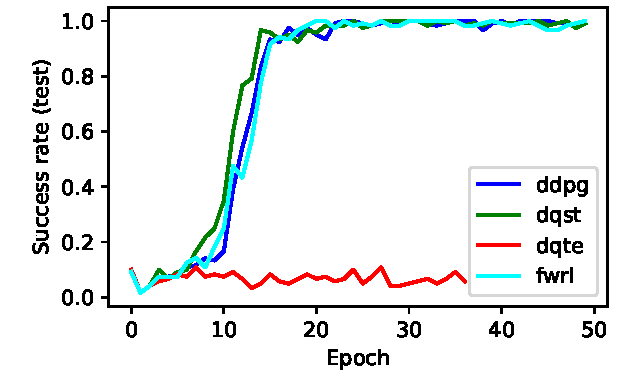
\includegraphics[width=\frac\columnwidth]{media/res/38f4625-FetchPush-v1-fwrl-future/test/success_rate.pdf}%
  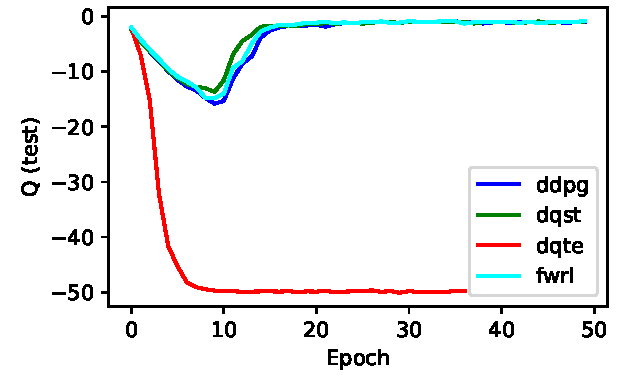
\includegraphics[width=\frac\columnwidth]{media/res/38f4625-FetchPush-v1-fwrl-future/test/mean_Q.pdf}%
  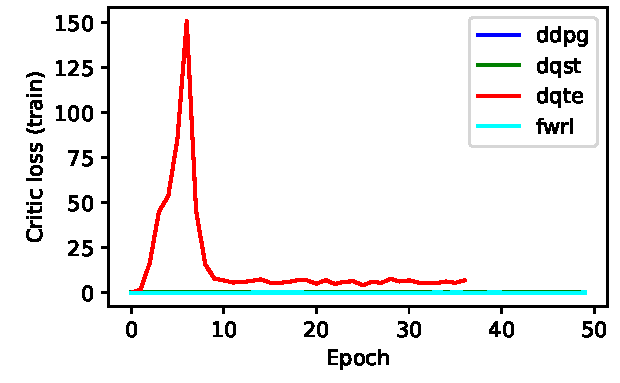
\includegraphics[width=\frac\columnwidth]{media/res/38f4625-FetchPush-v1-fwrl-future/train/critic_loss.pdf}\\
  On Fetch Reach\\
  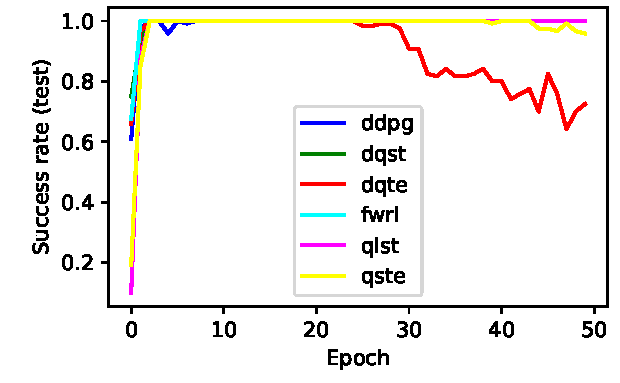
\includegraphics[width=\frac\columnwidth]{media/res/38f4625-FetchReach-v1-fwrl-future/test/success_rate.pdf}%
  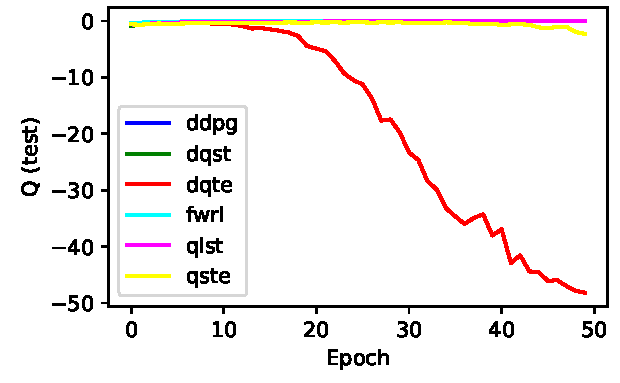
\includegraphics[width=\frac\columnwidth]{media/res/38f4625-FetchReach-v1-fwrl-future/test/mean_Q.pdf}%
  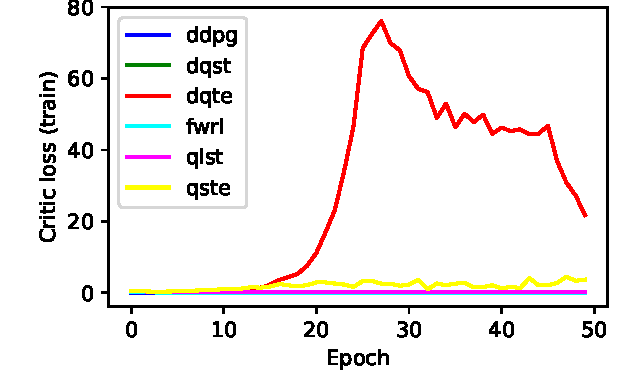
\includegraphics[width=\frac\columnwidth]{media/res/38f4625-FetchReach-v1-fwrl-future/train/critic_loss.pdf}\\
  On Fetch Slide\\
  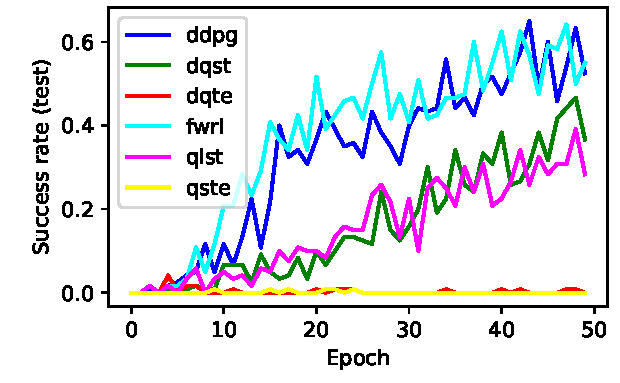
\includegraphics[width=\frac\columnwidth]{media/res/38f4625-FetchSlide-v1-fwrl-future/test/success_rate.pdf}%
  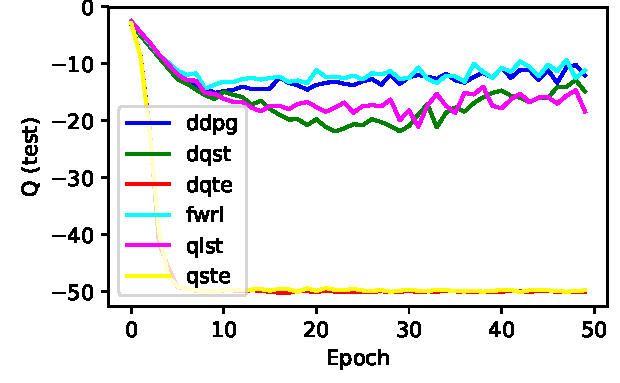
\includegraphics[width=\frac\columnwidth]{media/res/38f4625-FetchSlide-v1-fwrl-future/test/mean_Q.pdf}%
  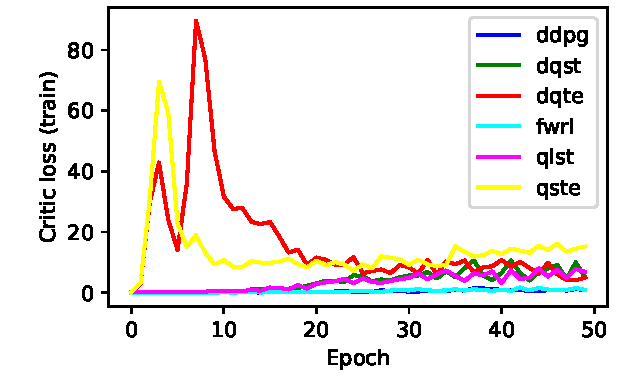
\includegraphics[width=\frac\columnwidth]{media/res/38f4625-FetchSlide-v1-fwrl-future/train/critic_loss.pdf}%
  \caption{
    Fetch results. Loss function changes do no seem to make a difference.
    There are four parts to the loss function (1) DDPG Loss $\Loss_{\text{ddpg}}$ ,
    (2) Step loss$\Loss_{\text{step}}$,  
    (3) Lower bound $\Loss_{\text{lower}}$ and
    (4) Upper bound $\Loss_{\text{upper}}$ .
    ddpg = $\Loss_{\text{ddpg}}$,
    dqst = $\Loss_{\text{ddpg}}$ + $\Loss_{\text{step}}$,
    fwrl = $\Loss_{\text{ddpg}}$ + $\Loss_{\text{lower}}$ +
    $\Loss_{\text{upper}}$,
    qlst = $\Loss_{\text{ddpg}}$ + $\Loss_{\text{step}}$ + $\Loss_{\text{lower}}$ + $\Loss_{\text{upper}}$,
    dqte = $\Loss_{\text{ddpg}}$ + $\Loss_{\text{trieq}}$,
    qste = $\Loss_{\text{ddpg}}$ + $\Loss_{\text{step}}$ + $\Loss_{\text{trieq}}$.
    Success rate is the fraction of times the agent reaches the goal. Q(test) is
    the estimated cumulative reward by the network. Critic loss is the total
    loss plotted during training.
    Because stfw, stlo, stup fail to succeed, we infer that the $\Loss_{\text{ddpg}}$ DDPG loss is
    critical for making the algorithm work. Since the qlst works better than
    fwrl, we infer that $\Loss_{\text{step}}$ Step loss is also important.
    only.
    Since there is slight improvement in dqst over ddpg, this means
    $\Loss_{\text{step}}$ really helps. dqst did not run fully but it shows
    promise (I need to fix a bug).
    But why does the loss for stfw keep rising? Does it mean that the SGD is not
    able to optimize the loss gradients in the right direction?
  }%
  \label{fig:fwrl-stepfwrl-noop-FetchPush}%
\end{figure}%
% 


%\subsection{Unanswered questions and things to try}
%
%\subsubsection{FWRL specific sampling}
%Right now the shuffle step in the algorithm is totally random and probably
%introduces more noise in the algorithm than it helps. A modification of HER
%sampling would sampling three time steps from the trajectory (single episode)
%$t_1 > t_2 > t_3$ and use $t_2$ as the intermediate state for
%$\Loss_{\text{upper}}$ and $\Loss_{\text{lower}}$.
%
%
%\subsubsection{Why is any loss term with upper/lower worse?}
%This is probably answered by  the above section but what are the other
%explanations. The total ``Critic loss'' is increasing for stfw
%($=\Loss_{\text{step}}$ + $\Loss_{\text{lower}}$ + $\Loss_{\text{upper}}$),
%which seems to say that with $\Loss_{\text{ddpg}}$, it is hard to optimize the functions.
%
%
%\subsection{Is it still a contribution if the upper and lower bounds do not
%  improve the results?}
%Can we claim that this alternative formulation is new and more principled than HER?


\section{Results}
\subsubsection{Quantitative Results}
We evaluate Q-learning Concatenated (QLCAT), Q-learning (QL), model-based RL
(MBRL) and Floyd-Warshall Reinforcement Learning (FWRL) on two metrics in two
different environments. The two metrics we use are Distance inefficiency and
average reward per episode. The baselines and metrics are explained in the
experiment section~\ref{sec:experiments}. The results are shown in
Figure~\ref{fig:ql-fw-grid-world-results}-\ref{fig:ql-fw-windy-world-rewards} 
We find that FWRL consistently achieves higher rewards, and lower distance
inefficiency than the baselines. The reward curves also show that FWRL learns to
find the higher reward much faster than the baselines, demonstrating higher
sample efficiency.

\begin{figure}%
  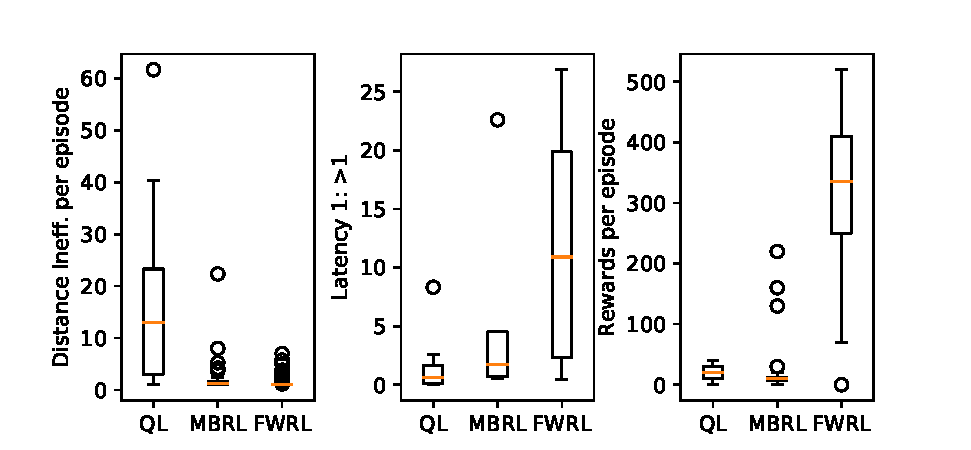
\includegraphics[width=\columnwidth]{./media/metrics-grid-world.pdf}{a}
  \caption{Results on grid world. FWRL beats Q-Learning
    consistently. Lower is better for Distance-Inefficiency. Higher
    is better for reward per episode. }
  \label{fig:ql-fw-grid-world-results}%
\end{figure}

\begin{figure}
  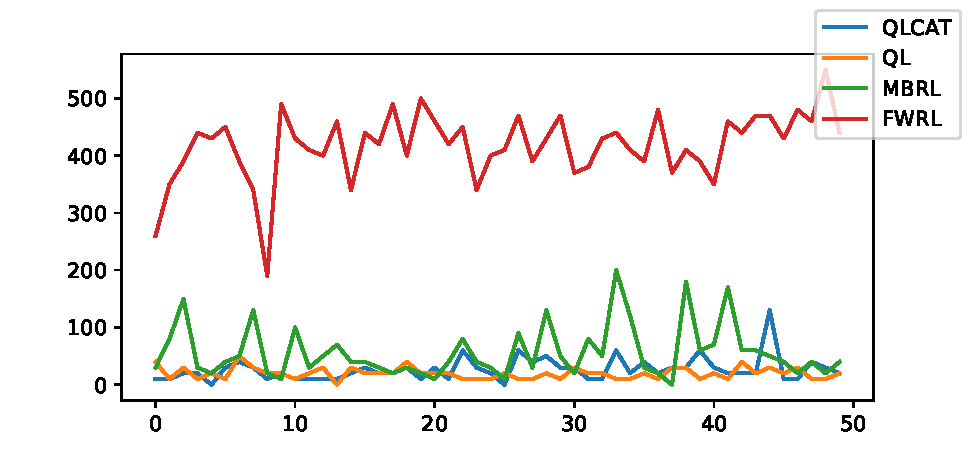
\includegraphics[width=\columnwidth]{./media/rewards-metrics-grid-world.pdf}{b}
  \caption{Reward curves on grid world. FWRL reward climbs much
    faster than all other baselines showcasing the improved \emph{sample
      efficiency} of the algorithm.}
  \label{fig:ql-fw-grid-world-reward-curves}%
\end{figure}

\begin{figure}
  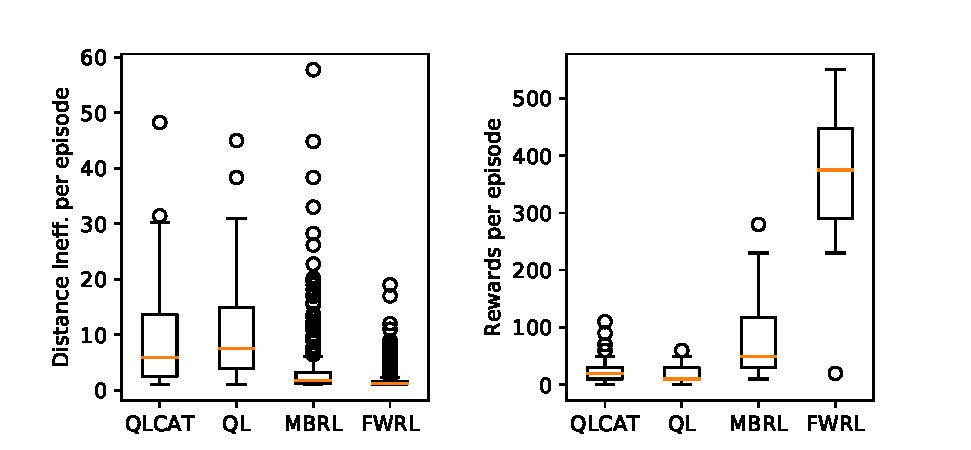
\includegraphics[width=\columnwidth]{./media/metrics-windy-world.pdf}
  \caption{Results on windy world. FWRL beats Q-Learning
    consistently. Lower is better for Distance-Inefficiency. Higher
    is better for reward per episode. }
  \label{fig:ql-fw-windy-world-results}%
\end{figure}

\begin{figure}
  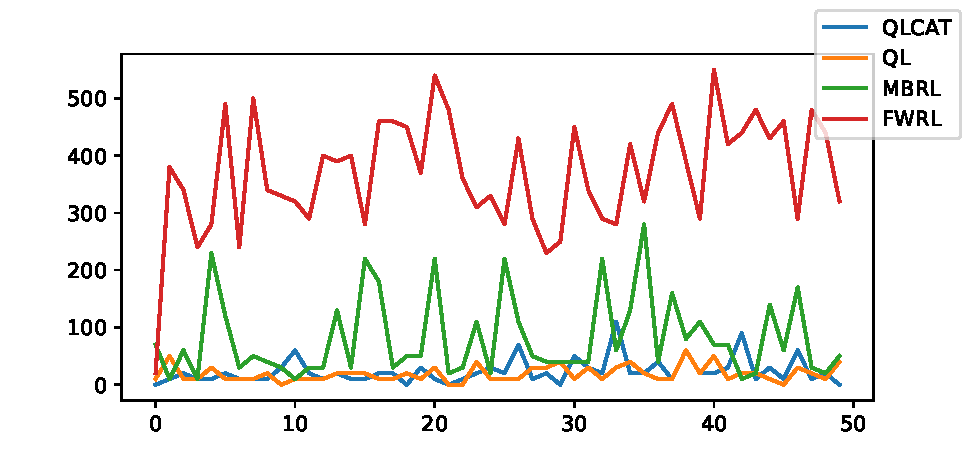
\includegraphics[width=\columnwidth]{./media/rewards-metrics-windy-world.pdf}
  \caption{Reward curves on windy world. FWRL reward climbs much
    faster than all other baselines showcasing the improved \emph{sample
      efficiency} of the algorithm.}
  \label{fig:ql-fw-windy-world-reward-curves}%
\end{figure}


\subsubsection{Qualitative Results}
To demonstrate the claim made in Fig~\ref{fig:visual-abstract}, we train QLCAT
and FWRL for two episodes each with start and goal locations such that the path
meets in the center. Unlike quantitative experiments, in this experiment the
episode ends when the agent reaches the goal.
After two episodes of training, in which both FWRL (Floyd-Warshall RL) and QLCAT
(Q-Learning with goal concatenated to the state) reach the desired
goals via exploration, we put the algorithms to test.
For the test episode, the goal is chosen from first training episode but start
location is chosen from second training episode.
During the test episode,
we turn off $\epsilon$-greed exploration and follow the greedy policy.

We find that QLCAT decides to repeat the action that pushes it into the wall,
therefore is unable to move. However, FWRL reaches the goal using the shortest
path. The trajectories and value functions are visualized in Figure~\ref{fig:qualitative-results}.

\begin{figure}
  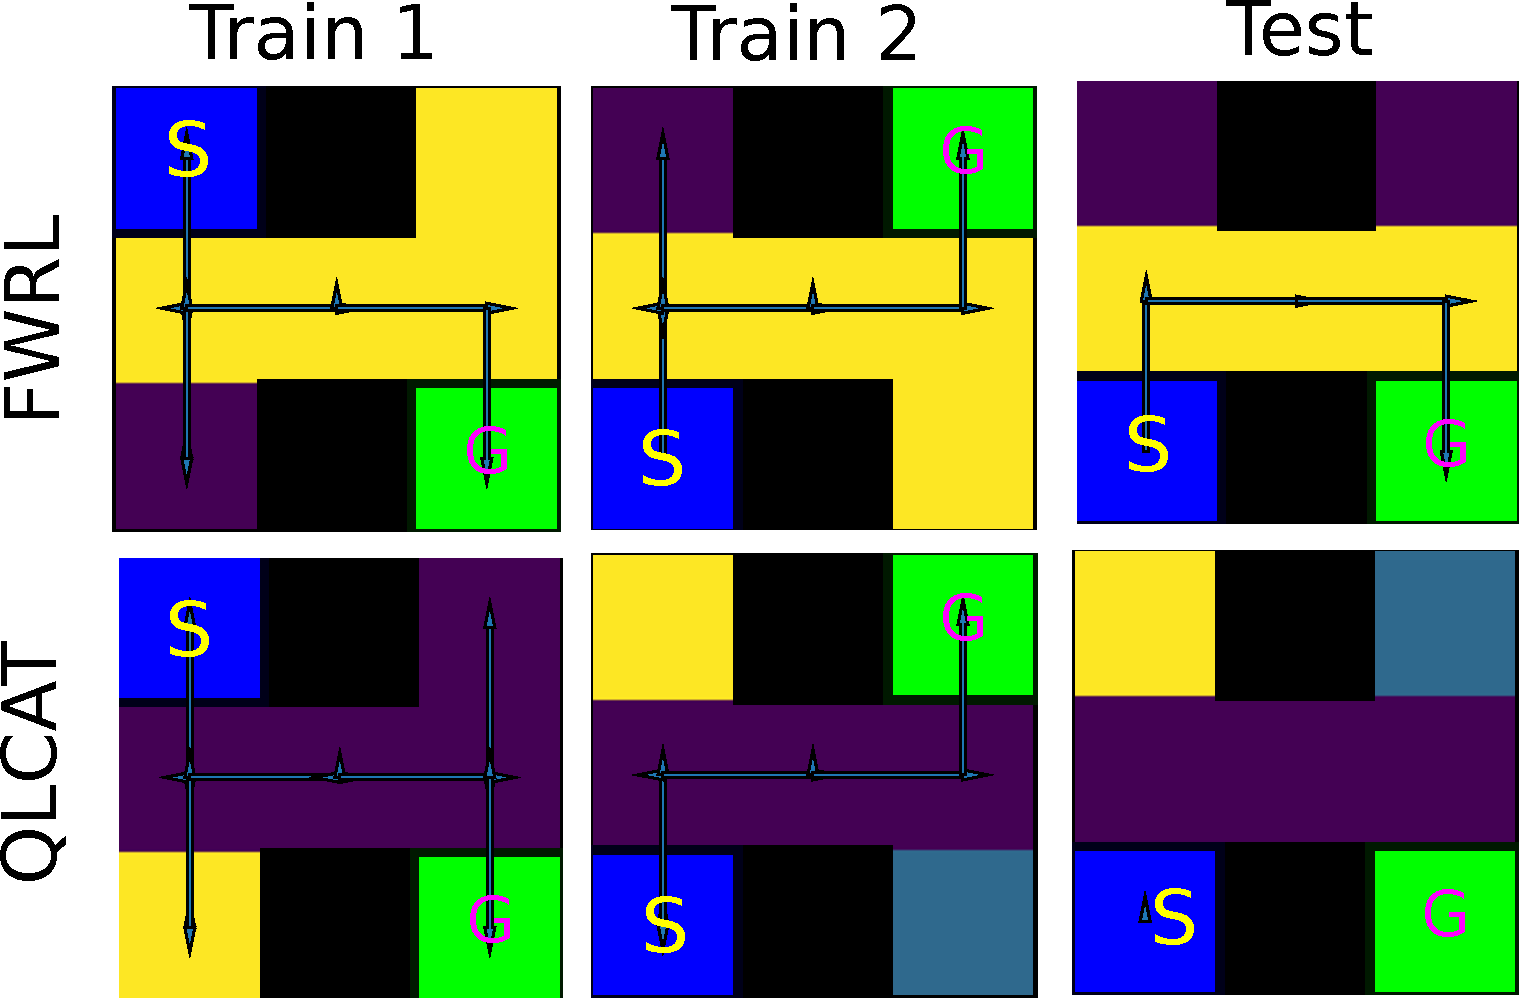
\includegraphics[width=\columnwidth]{./media/qualitative-results.pdf}
  \caption{Qualitative results: Visualization of value-function in H-Maze. Green
box with G represents goal location, Blue box with S represents start location.
The obstacles are shown black. The trajectories are shown by arrows. The color
of remaining boxes show the expected value of each state computed by the
corresponding algorithm. Each row different algorithm, while columns show
different episodes. We find that QLCAT is unable to learn a new trajectory
when given an unseen combination of start and end location. FWRL (ours) finds the
shortest path easily in such a test case. }
\label{fig:qualitative-results}
\end{figure}


\section{Ablation Studies}I



\section{Related Work}


The recent surge in popularity of reinforcement learning occured with
the introduction of \emph{Deep Q Networks} which
learned to play atari video games from raw pixel values while beating
human players \citep{mnih2013playing}. Subsequently,
DQNs saw

Goal-conditioned value functions have been explored extensively in the
literature. Our work builds of the formulation of \emph{Universal Value Function
Approximators}\cite{schaul2015universal}.  


\subsection{Experience Replay and Target Networks}
The use of \emph{experience replay} to learn from off-policy experiences
and and slower-changing \emph{target
networks} are fundamental to the succesful operation of DFWRL. Both
methods were popularized for use in the DRL literature in
\citet{mnih2015human}'s original DQN work. 

\subsection{Curriculum Learning}
Curriculum learning, first introduced by \citet{bengio2009curriculum},
operates on the simple assumption that learning can in complex domains
can be achieved by first iterating over simpler variants of the problem.
This work builds of \emph{Hindsight Experience Replay}
\citep{andrychowicz2017hindsight}, a form of \emph{implicit curriculum}
wherein past failed experiences are relabelled with goal states that in
turn significantly accelerates learning. 


\subsection{Goal conditioned value functions}
Several variants of goal-conditioned value functions have been explored
extensively in the literature
\citep{sutton2011horde,schaul2015universal}.  Driven by the idea that
simulataneously learning several tasks leads to better generalizability
than learning a single tasks \citep{pong2018temporal}, goal-conditioned
value functions have been shown to possess value in manipulation
\citep{plappert2018multi,peng2018sim} and navigation domains
\citep{zhang2017deep,mirowski2018learning}. Aside from Dhiman et. al.,
while much work has utilized these specialized value functions to learn
how to solve complicated tasks, we were unable to find any other work
that leveraged the structure in the space of these functions to
accelerate and improve learning. 


\subsection{Multi-goal Reinforcement Learning Methods (HER/TDM)}
Learning goal-conditioned value functions have also taked a variety of
forms. In \emph{model-free} RL, \emph{Hindsight Experience Replay} (HER)
\citep{andrychowicz2017hindsight} represents a form of \emph{implicit
curriculum} for training these functions. In HER, previous traversals
are re-used for training with the goal state relabelled to be a part of
these state traversals. HER sampling is shown to be highlight effective
in training goal-conditioned value functions quickly and efficiently and
is highly influential on our methods. In
\emph{model-based} RL, \emph{Temporal Difference Models}
\citep{pong2018temporal} derive a
connection between model-based and model-free algorithms for
finite-horizon problems. TDM's define and learn goal and
horizon-conditioned value functions and showcase improved performance
over scores and sample efficiencies over model-based baselines while
retaining the asymptotic performance of model-free RL. Being exclusively
\emph{model-free} and horizon-independent, DFWRL represents an
orthogonal direction of research as compared to TDMs. 




\section{Conclusion}
In this work we pose a reinterpretation of goal conditioned value
functions and show that under this paradigm learning is possible in the
absence of goal reward. This is a a suprising result that runs counter
to intuitions that underly most reinforcement learning algorithms.  

Since our method cannot recognized locations that close to the desired
location, in future work we wish to extend our formulation to
incorporate the distance-threshold. We also wish to improve the
the performance FWRL on deep neural networks. 

We hope that the experiments and results presented in this paper  lead
to a broader discussion about the assumptions actually required for
learning multi-goal tasks.


%\begin{algorithm}
  \tcc{By default all states are unreachable}
  Initialize $\fwargs{\state_i}{\act_i ; \param_{\fwcost}}{\state_j}{}{} \leftarrow -\infty$ \;

  Define $\policy^*(\state_t, \state_g, \fw) = \arg \max_{\act}
  \fwargs{\state_t}{\act; \param_{\fwcost}}{\state_g}{}{}$ \;
  % We do not know the goal location
  Input $\state_g$ \;
  Set $t \leftarrow 0$\;
  Observe $\state_t$ \;
  \For{$t \leftarrow 1$ \KwTo $\epiT$}{
    Take action $\act_{t} \sim \epsilon\text{-greedy}(\policy^*(\state_{t}, \state_g, \fw))$ \;
    Observe $\state_{t+1}$, $\rew_t$ \;
    \If{$\rew_t >= \Rgoal$}{
        %\tcc{Note the goal state}
      %$\state_g \leftarrow \state_t$ \;
      \tcc{Do not update the value function with goal reward}
      continue\;
    }
    % Update the transition reward
    $\fwargs{\state_{t}}{\act_{t}}{\state_{t+1}}{}{} \leftarrow \rew_t$ \;
    \For{$\state_k \in \State, \act_k \in \Act, \state_l \in \State$}{
      $\fwargs{\state_k}{\act_k}{\state_l}{}{} \leftarrow
        \max \{
        \fwargs{\state_k}{\act_k}{\state_l}{}{},
        \fwargs{\state_k}{\act_k}{\state_t}{}{}
        + \max_{\act_p \in \Act} \fwargs{\state_t}{\act_p}{\state_l}{}{}
        \}$
        \;
    }
  }
  \KwResult{$\policy^*(\state_k, \state_g, \fwcost)$}
  \caption{\small Floyd-Warshall Reinforcement Learning (Tabular setting)}
  \label{alg:floyd-warshall-small}
\end{algorithm}


%\begin{function}
%\eIf{$\state_g = \phi$ or $\text{all}(\fwcost(\state_t, :, \state_g) = -\infty)$ }{
%  \tcc{Exploration mode}
%  $\act^* = \arg\max_{\act} Q(\state_t, \act)$\;
%}{
%  \tcc{Exploitation mode}
%  $\act^* = \arg\max_{\act} F(\state_t, \act, \state_g)$\;
%}
%
%\caption{Policy()}%$\policy^*(\state_t, \state_g, Q(., .), \fwcost(.,.,.))$}
%\label{func:policy}
%\KwRet{$\act^*$}
%\end{function}


%
%\subsection{Future work}
%Items to improve the algorithm:
%\begin{itemize} \item
%\TODO{Justify the computational cost of constraint} The cost of going through the entire state space.
%How do you extend to a network? and large state spaces.
%\begin{enumerate}\item
%Observation 1: If there is only one goal, then the computation should not be any more than Q-learning.
%This can be accomplished by assuming that transitivity is satisfied till
%$\state_{t-1}$ and needs to be extend to only the next step. This sounds similar to the
% Floyd-Warshall dynamic programming update.
%However, this assumes that $\state_t$ is being visited for the first time.
%If the state $\state_t$ is being visited for the second time, the earlier
%value may be the shorter path for it.
%\end{enumerate}
%\item
%We need Q-value for exploration.
%\end{itemize}



\def\localbib{/home/dhiman/wrk/group-bib/shared}
\IfFileExists{\localbib.bib}{
\bibliography{\localbib,main,main_filtered}}{
\bibliography{main,main_filtered}}
\bibliographystyle{iclr2019_conference}

\section{Appendix}

Our algorithm~\ref{alg:floyd-warshall-deep} is different from
HER~\cite{andrychowicz2016learning} because it contains additional step-loss
term $\LossStep$ at line number 17 which allows the algorithm to learn even when
the rewards received are independent of desired goal. Also in HER sampling (line
13), the algorithm recomputes the rewards because the goal is replaced with a
pseudo-goal. Our algorithm does not need reward recomputation because the reward
formulation does not depend on the goal and is not affected by choice of
pseudo-goal.

Our algorithm is also different from Floyd-Warshall Reinforcement learning
because it does not contain $\LossUp$ and $\LossLo$ terms and contains the
additional $\LossStep$.

\begin{algorithm}
  \tcc{By default all states are unreachable}
  Initialize networks
  $\fwargs{\state_i}{\act_i }{\goal_j; \param_{\fwcost}}{*}{}$ and
  $\policy(\state_i, \state_g; \param_{\policy})$ \;
  Copy the main network to target network
  $\fwargs{\state_i}{\act_i ;\param_{\fwcost}}{\state_j}{t}{} \leftarrow
  \fwargs{\state_i}{\act_i ; \param_{\fwcost}}{\state_j}{*}{} $ \;

  % We do not know the goal location
  Initialize replay memory $M$ \;
  \tcc{Collect experience}
  \For{$e \leftarrow 1$ \KwTo $M$}{
    Sample $\goal_e \in \Goal$ \;
    Set $t \leftarrow 0$\;
    Observe state $\state_t$ and achieved goal $\goal_t$ \;
    \For{$t \leftarrow 1$ \KwTo $\epiT$}{
      Take action $\act_{t} \leftarrow \epsilon\text{-greedy}(\policy(\state_{t}, \goal, \fw))$ \;
      Observe $\state_{t+1}, \goal_{t+1}, \rew_t$ \;
      Store $(\state_{t}, \goal_t, \act_t, \state_{t+1}, \goal_{t+1}, \rew_t; \goal_e)$ in memory $M[e]$ \;
    }
    
    \tcc{Train}
    \For{$t \leftarrow 1$ \KwTo $\epiT$}{
      % Update the transition reward
      
      HER sample batch $B = [
      (\state_{i}, \goal_i, \act_i, \state_{i+1}, \goal_{i+1}, \rew_i;
      \goal_{i+f_i}),
      \dots ,
      (\state_{b}, \goal_b, \act_b, \state_{b+1}, \goal_{b+1}, \rew_b; \goal_{b+f_b})]$ from $M$ \;
      $\Loss(\dots) = 0$ \;
      \For{$b \in B$}{
        $(\state_{b}, \goal_b, \act_b, \state_{b+1}, \goal_{b+1}, \rew_b, \goal_{b+f_b}) = B[b]$ \;
        $\Loss(\dots) += (\fwargs{\state_{b}}{\act_{b}}{\goal_{b+1}}{*}{} - \rew_b)^2$ 
        \tcc*{Step loss}
        $\Loss(\dots) += (\fwargs{\state_{b}}{\act_{b}}{\goal_{b+f_b}}{*}{} -
        \rew_b - \discount\fwargs{\state_{b+1}}{\policy_t(\state_{b+1}, \goal_{b+f_b};\param_\policy)}{\goal_{b+f_b}}{t}{})^2$
        \tcc{DDPG loss}
      }
      Update gradients for $\fw_*$ and $\policy$ using loss $\Loss(\dots)$\;
    }
  }
  \KwResult{$\policy^*(\state_k, \state_g, \fwcost)$}
  \caption{\small Path-reward reinforcement learning}
  \label{alg:floyd-warshall-deep}
\end{algorithm}


%\begin{function}
%\eIf{$\state_g = \phi$ or $\text{all}(\fwcost(\state_t, :, \state_g) = -\infty)$ }{
%  \tcc{Exploration mode}
%  $\act^* = \arg\max_{\act} Q(\state_t, \act)$\;
%}{
%  \tcc{Exploitation mode}
%  $\act^* = \arg\max_{\act} F(\state_t, \act, \state_g)$\;
%}
%
%\caption{Policy()}%$\policy^*(\state_t, \state_g, Q(., .), \fwcost(.,.,.))$}
%\label{func:policy}
%\KwRet{$\act^*$}
%\end{function}

\section{Ablation on loss and goal rewards}

In Figure~\ref{fig:loss-ablation} and Figure~\ref{fig:path-rewards} we show
ablation on loss functions and goal rewards. In Figure~\ref{fig:path-rewards}
Our method is shown in blue with HER - Goal rewards + $\LossStep$.

\begin{figure*}
%\begin{figure}
%\begin{wrapfigure}[19]{r}{0.5\columnwidth}
\begin{minipage}[t]{0.45\linewidth}
\begin{tikzpicture}
  \def\resultsdir{DhBaSiCoICLR2019/media/res}
  \begin{axis}[ymin=0,xmin=0,
  xlabel=Epochs,
  width=1.0\columnwidth,
  height=0.70\columnwidth,
  every axis plot/.append style={line width=1.0pt},
  legend style={fill=none,font=\sffamily\fontsize{2.9}{4}\selectfont},
  ylabel=Success Rate (test),
  legend pos=north west]
\addplot table [x=epoch, y=test/success_rate, col sep=comma] {\resultsdir/3f1eafe-FetchPush-v1-qlst-future/progress.csv};
\addlegendentry{HER $+ \LossStep + \LossLo + \LossUp$};
\addplot table [x=epoch, y=test/success_rate, col sep=comma] {\resultsdir/3f1eafe-FetchPush-v1-stfw-future/progress.csv};
\addlegendentry{HER - $\LossDDPG + \LossStep + \LossLo + \LossUp$};
\addplot table [x=epoch, y=test/success_rate, col sep=comma] {\resultsdir/3f1eafe-FetchPush-v1-fwrl-future/progress.csv};
\addlegendentry{HER $ + \LossLo + \LossUp$};
% This experiment did not run full. Replaced with same parameters.
%\addplot table [x=epoch, y=test/success_rate, col sep=comma] {\resultsdir/3f1eafe-FetchPush-v1-dqst-future/progress.csv};
%\addlegendentry{HER $ + \LossStep$};
\addplot table [x=epoch, y=test/success_rate, col sep=comma] {\resultsdir/be0910c-her_fwrl_path_reward-FetchPush-v1-dqst/progress.csv};
\addlegendentry{HER $ + \LossStep$};
\addplot table [x=epoch, y=test/success_rate, col sep=comma] {\resultsdir/3f1eafe-FetchPush-v1-stlo-future/progress.csv};
\addlegendentry{HER $ + \LossLo$};
\addplot table [x=epoch, y=test/success_rate, col sep=comma] {\resultsdir/3f1eafe-FetchPush-v1-stup-future/progress.csv};
\addlegendentry{HER $ + \LossUp$};
\addplot table [x=epoch, y=test/success_rate, col sep=comma] {\resultsdir/3f1eafe-FetchPush-v1-ddpg-future/progress.csv};
\addlegendentry{HER};
\end{axis}
\end{tikzpicture}
\caption{Ablation on loss functions for Fetch Push task. The
  Floyd-Warshall inspired loss functions $\LossLo$ and $\LossUp$ do not help
  much. $\LossStep$ helps a little but only in conjunction with HER~\cite{andrychowicz2016learning}.}
\label{fig:loss-ablation}
%\end{figure}%
%\end{wrapfigure}%
\end{minipage}\hfill
%\begin{figure}
%\begin{wrapfigure}[16]{r}{0.5\columnwidth}
\begin{minipage}[t]{0.45\linewidth}
\newcommand{\xcol}{epoch}
%\newcommand{\ycol}{test/ag_g_dist}
\newcommand{\ycol}{test/success_rate}
\begin{tikzpicture}
  \def\resultsdir{media/res}
  \begin{axis}[ymin=0,xmin=0,
  xlabel=Epochs,
  width=1.0\columnwidth,
  height=0.70\columnwidth,
  ylabel=Success Rate (test),
  every axis plot/.append style={line width=1.0pt},
  legend style={fill=none,font=\sffamily\fontsize{3.0}{4}\selectfont},
  legend pos=south east]
\addplot table [x=\xcol, y=\ycol, col sep=comma] {\resultsdir/be0910c-her_fwrl_path_reward-FetchPush-v1-dqst/progress.csv};
\addlegendentry{HER $+\LossStep$};
\addplot table [x=\xcol, y=\ycol, col sep=comma] {\resultsdir/be0910c-her_fwrl_path_reward-FetchPushPR-v1-dqst/progress.csv};
\addlegendentry{HER - Goal reward $+\LossStep$};
\addplot table [x=\xcol, y=\ycol, col sep=comma] {\resultsdir/be0910c-her_fwrl_path_reward-FetchPushPR-v1-ddpg/progress.csv};
\addlegendentry{HER - Goal rewards};
\addplot table [x=\xcol, y=\ycol, col sep=comma] {\resultsdir/be0910c-her_fwrl_path_reward-FetchPush-v1-ddpg/progress.csv};
\addlegendentry{HER};
\end{axis}
\end{tikzpicture}
\caption{Even when the Goal rewards are removed from
  HER~\cite{andrychowicz2016learning} training, the HER
  is able to learn only if the $\LossStep$ is added again.
  (HER-Goal Rewards+$\LossStep$) is our proposed method.
}
\label{fig:path-rewards}
%\end{figure}%
%\end{wrapfigure}%
\end{minipage}
\end{figure*}

\newpage

\section{Old Experiments}
%
\subsection{Notation}

\begin{tabular}{ll}   
  \toprule
  Symbol & Meaning\\
  \midrule
  $\state \in \State$ & State $\state$ in state space $\State$ \\
  $\act \in \Action$ & Action $\act$ in Action space $\Action$ \\
  $\rew \in \R$ & Observed reward \\
  $\goal \in \Goal$ & Goal $\goal$ in goal space $\Goal$ \\
  $f_\goal(\state_t): \State \rightarrow \Goal$ & Function to compute achieved goal \\
  $\Rew(\state, \act) : \State \times \Action \rightarrow \R $ & Reward function \\
  $\Rew(\state, \goal, \act) : \State \times \Goal \times \Action \rightarrow \R $ & Goal-conditioned Reward function \\
  $\TransFull$ & Transition function \\
  $\discount$ & Discount factor \\
  MDP=$(\State, \Action, \Trans, \Rew, \discount)$& Markov Decision Process \\
  $\policy(\state): \State \rightarrow \Action $ & Policy function \\
  $\policy(\state, \goal): \State \times \Goal \rightarrow \Action $ & Goal conditioned Policy function \\
  $\Q_\policy(\state, \act; \param_\Q) = \E_\policy[ \sum_{k=t}^\infty \discount^{k-t} \Rew(\state_k, \act_k) | \state_t = \state, \act_t = \act ] $ & $Q$-function \\
  $\Q^*(\state, \act; \param_\Q) = \arg \max_\policy \Q_\policy(\state, \act; \param_\Q)$ & Optimal $Q$-function \\
  $\fwargs{\state}{\act}{\goal^*}{\policy}{} = \E_\policy[ \sum_{k=t}^\infty \discount^{k-t}\Rew(\state_k, \goal^*, \act_k) | \state_t = \state, \act_t = \act]$ & Goal conditioned Q-function \\
  \bottomrule
\end{tabular}
\begin{figure}%
  \def\frac{0.24}
  On Fetch Reach\\
  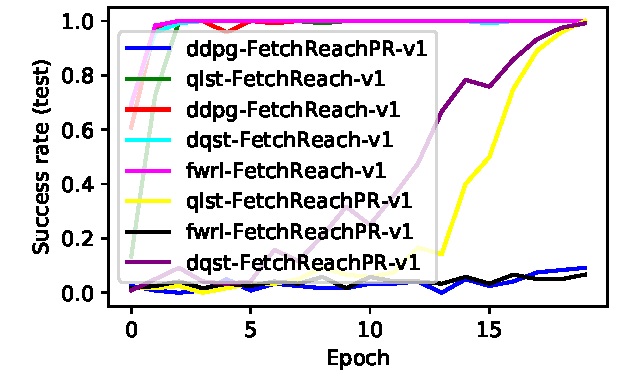
\includegraphics[width=\frac\columnwidth]{media/res/245b3c4-ce781a70-FetchReachPR-v1-fwrl-future-her_fwrl_path_reward/test/success_rate.pdf}%
  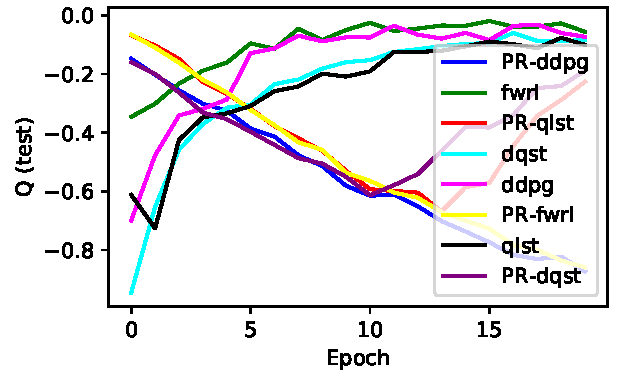
\includegraphics[width=\frac\columnwidth]{media/res/245b3c4-ce781a70-FetchReachPR-v1-fwrl-future-her_fwrl_path_reward/test/mean_Q.pdf}%
  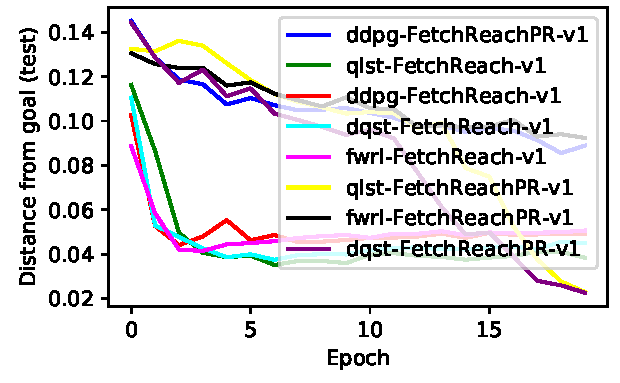
\includegraphics[width=\frac\columnwidth]{media/res/245b3c4-ce781a70-FetchReachPR-v1-fwrl-future-her_fwrl_path_reward/test/ag_g_dist.pdf}%
  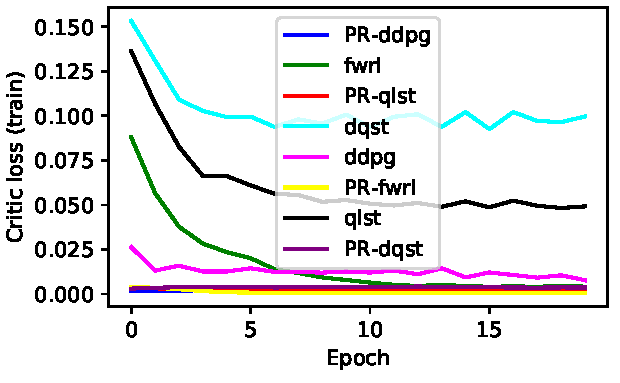
\includegraphics[width=\frac\columnwidth]{media/res/245b3c4-ce781a70-FetchReachPR-v1-fwrl-future-her_fwrl_path_reward/train/critic_loss.pdf}\\
  On Fetch Push\\
  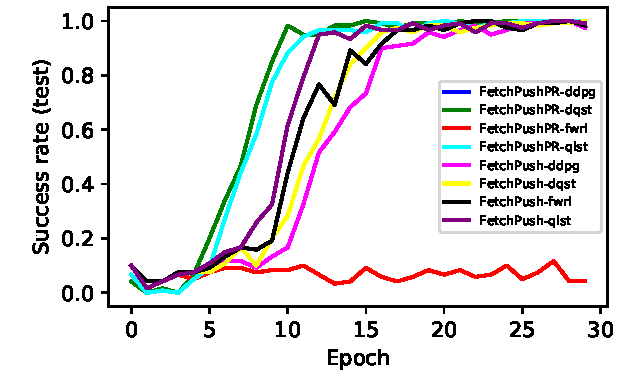
\includegraphics[width=\frac\columnwidth]{./media/res/be0910c-her_fwrl_path_reward-FetchPushPR-v1-fwrl/test/success_rate.pdf}%
  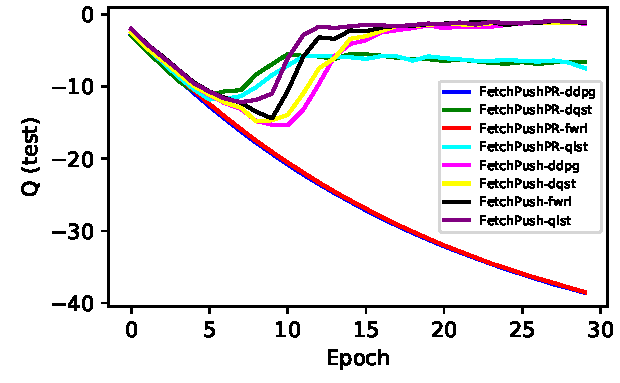
\includegraphics[width=\frac\columnwidth]{./media/res/be0910c-her_fwrl_path_reward-FetchPushPR-v1-fwrl/test/mean_Q.pdf}%
  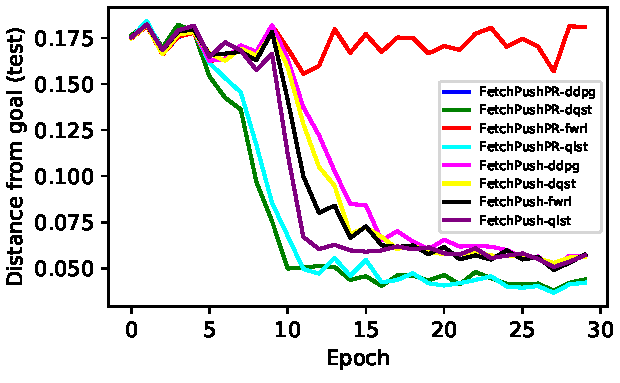
\includegraphics[width=\frac\columnwidth]{./media/res/be0910c-her_fwrl_path_reward-FetchPushPR-v1-fwrl/test/ag_g_dist.pdf}%
  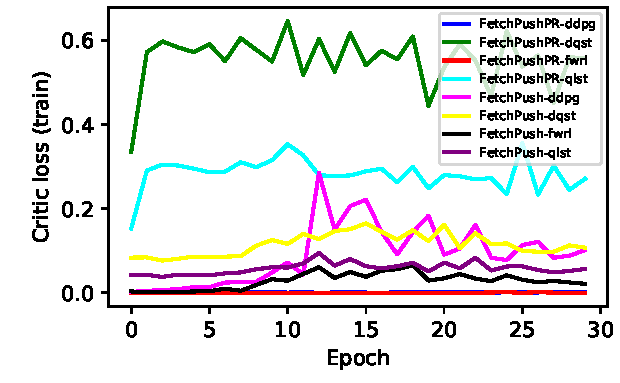
\includegraphics[width=\frac\columnwidth]{./media/res/be0910c-her_fwrl_path_reward-FetchPushPR-v1-fwrl/train/critic_loss.pdf}\\
  On Fetch Slide\\
  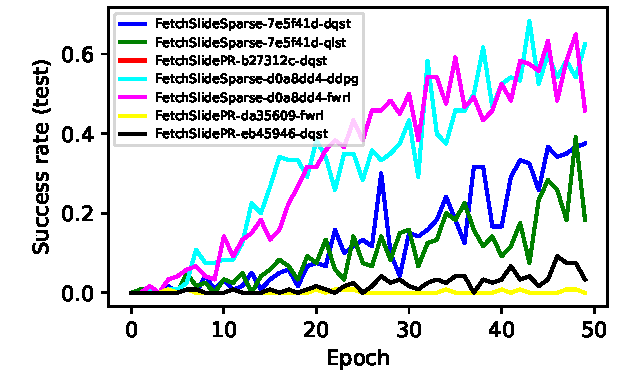
\includegraphics[width=\frac\columnwidth]{./media/res/eb45946-path_reward-FetchSlidePR-v1-dqst/test/success_rate.pdf}%
  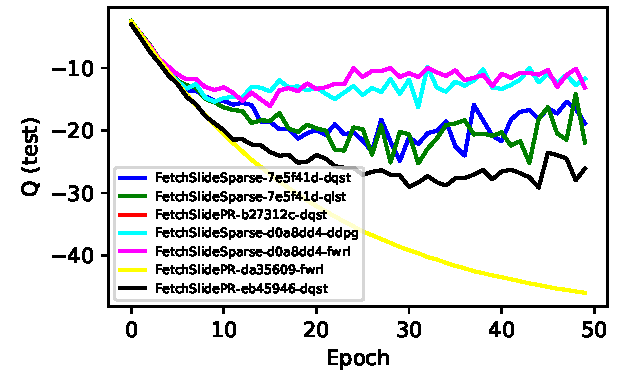
\includegraphics[width=\frac\columnwidth]{./media/res/eb45946-path_reward-FetchSlidePR-v1-dqst/test/mean_Q.pdf}%
  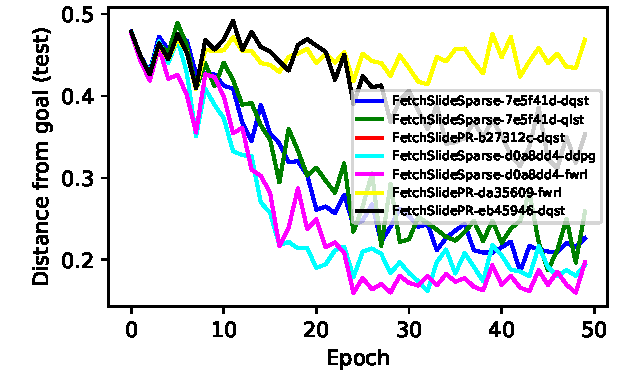
\includegraphics[width=\frac\columnwidth]{./media/res/eb45946-path_reward-FetchSlidePR-v1-dqst/test/ag_g_dist.pdf}%
  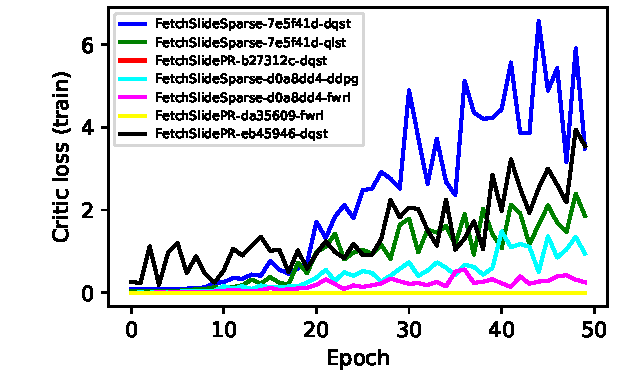
\includegraphics[width=\frac\columnwidth]{./media/res/eb45946-path_reward-FetchSlidePR-v1-dqst/train/critic_loss.pdf}\\
  On Fetch Pick And Place\\
  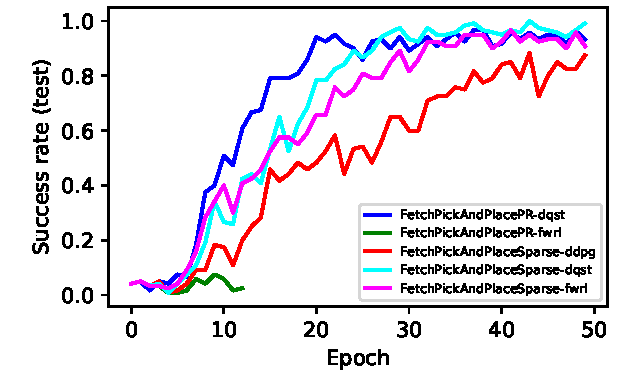
\includegraphics[width=\frac\columnwidth]{./media/res/d5cefef-path_reward-FetchPickAndPlacePR-v1-dqst/test/success_rate.pdf}%
  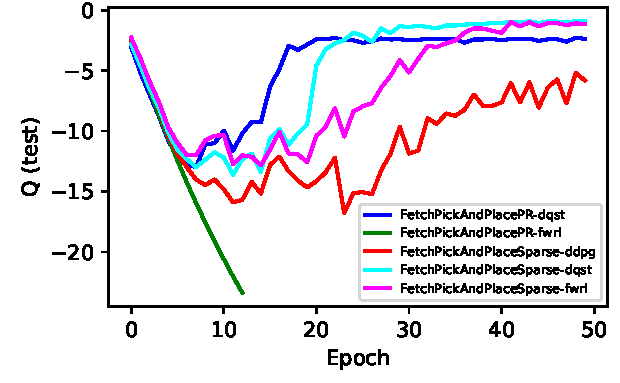
\includegraphics[width=\frac\columnwidth]{./media/res/d5cefef-path_reward-FetchPickAndPlacePR-v1-dqst/test/mean_Q.pdf}%
  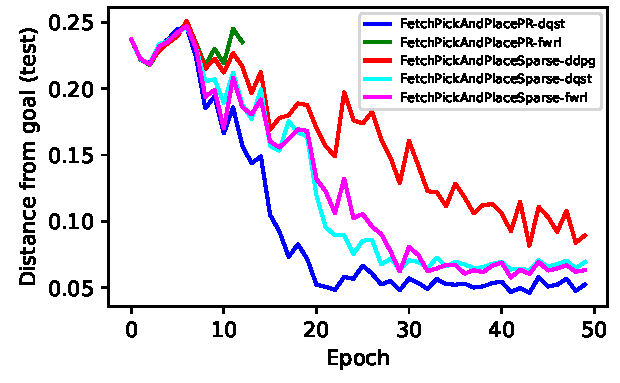
\includegraphics[width=\frac\columnwidth]{./media/res/d5cefef-path_reward-FetchPickAndPlacePR-v1-dqst/test/ag_g_dist.pdf}%
  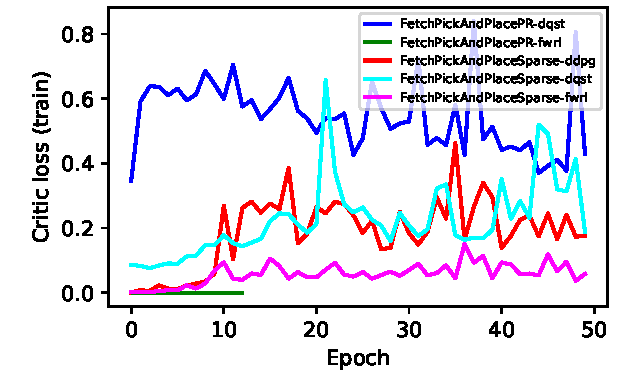
\includegraphics[width=\frac\columnwidth]{./media/res/d5cefef-path_reward-FetchPickAndPlacePR-v1-dqst/train/critic_loss.pdf}\\
  On Hand Reach \\
  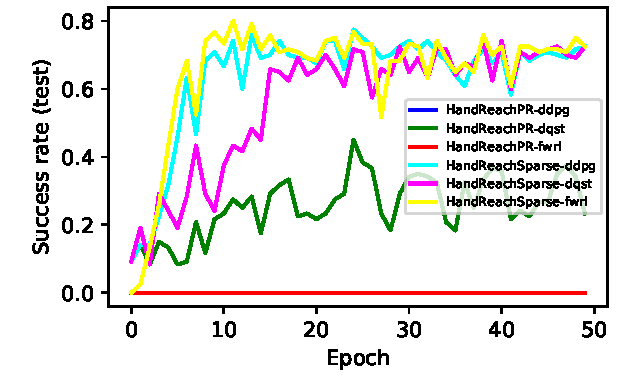
\includegraphics[width=\frac\columnwidth]{./media/res/d5cefef-path_reward-HandReachPR-v0-dqst/test/success_rate.pdf}%
  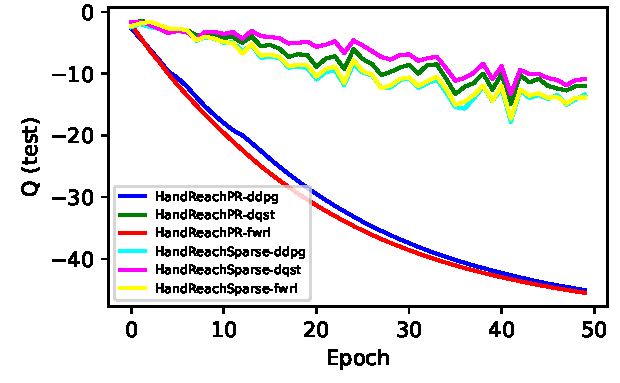
\includegraphics[width=\frac\columnwidth]{./media/res/d5cefef-path_reward-HandReachPR-v0-dqst/test/mean_Q.pdf}%
  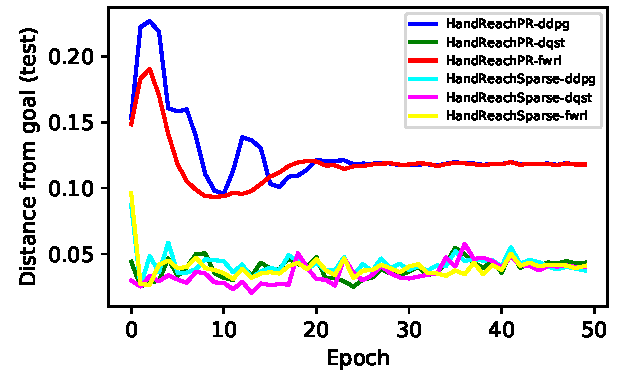
\includegraphics[width=\frac\columnwidth]{./media/res/d5cefef-path_reward-HandReachPR-v0-dqst/test/ag_g_dist.pdf}%
  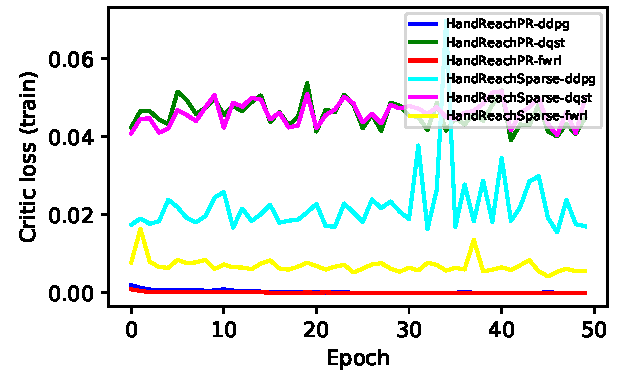
\includegraphics[width=\frac\columnwidth]{./media/res/d5cefef-path_reward-HandReachPR-v0-dqst/train/critic_loss.pdf}\\
  \label{fig:path-reward-1}%
  \caption{Effect of path reward on convergence in case of different loss
    functions on FetchReach. With path reward on PR-dqst
    ($\LossDDPG$ + $\LossStep$)
    and PR-qlst
    ($\LossDDPG$ + $\LossStep$ + $\LossLo$ + $\LossUp$), are able achieve high
    success rate and even that takes longer than usual. Out of the two PR-dqst
    does better. The terms with PR use path-rewards and hence less computation
    by avoid recomputation of reward function. It is interesting that PR-dqst
    and PR-qlst reach closer in terms of distance from goal probably because of
    absence of threshold.}%
\end{figure}%
% 

\begin{figure}
  \def\frac{0.32}
    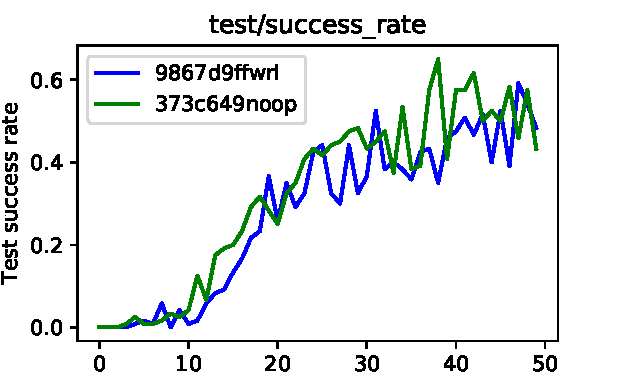
\includegraphics[width=\frac\columnwidth]{media/res/373c649_FetchSlide-v1-noop/test/success_rate.pdf}%
    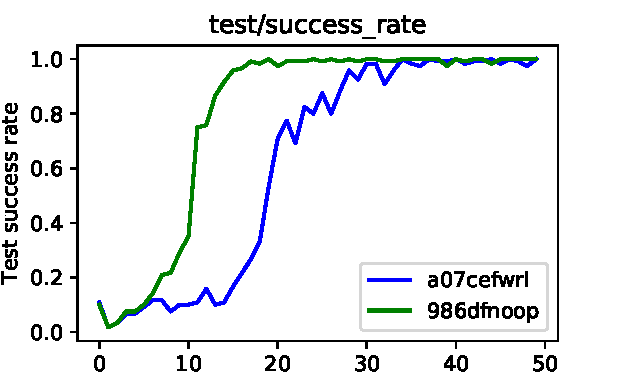
\includegraphics[width=\frac\columnwidth]{media/res/a077c9e_FetchPush-v1-fwrl/test/success_rate.pdf}%
    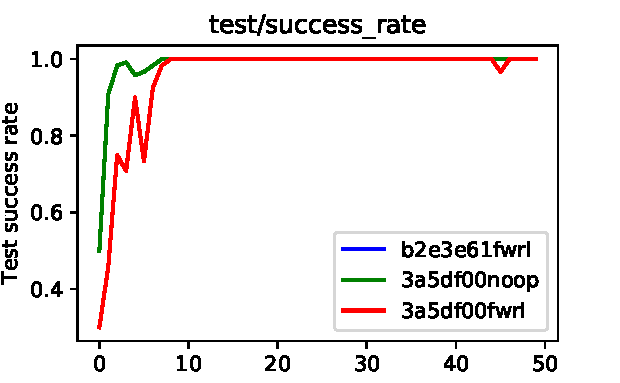
\includegraphics[width=\frac\columnwidth]{media/res/3a5df00_FetchReach-v1-fwrl/test/success_rate.pdf}\\
    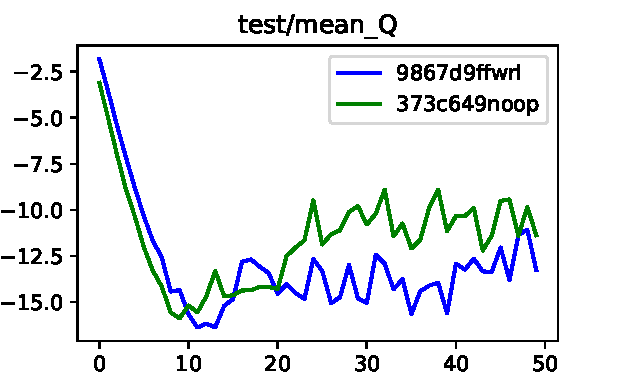
\includegraphics[width=\frac\columnwidth]{media/res/373c649_FetchSlide-v1-noop/test/mean_Q.pdf}%
    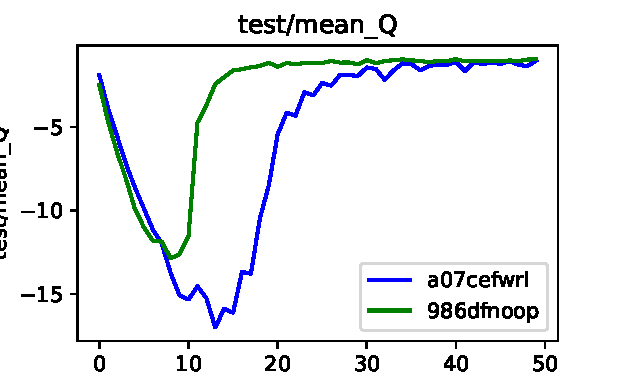
\includegraphics[width=\frac\columnwidth]{media/res/a077c9e_FetchPush-v1-fwrl/test/mean_Q.pdf}%
    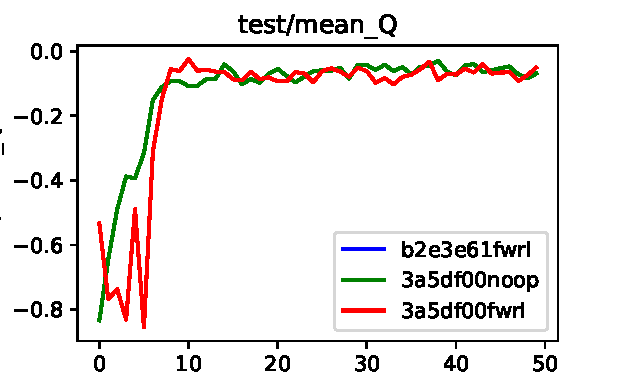
\includegraphics[width=\frac\columnwidth]{media/res/3a5df00_FetchReach-v1-fwrl/test/mean_Q.pdf}
    \caption{fwrl = Floyd Warshall ($=\Loss_{\text{ddpg}} +
      \Loss_{\text{upper}}$) with HER sampling;
      noop = DDPG ($=\Loss_{\text{ddpg}}$)with HER sampling.
  Test success rate and Mean Q on (1) Fetch-Slide, (2) Fetch-Push and (3)
  Fetch-Reach task. fwrl does consistently worse than HER.}
    \label{fig:fetch-slide-success}
\end{figure}


%
\begin{figure}%
  \def\frac{0.24}
  With HER sampling:\\
  \includegraphics[width=\frac\columnwidth]{media/res/3a90344-FetchReach-v1-stepfwrl-future/test/success_rate.pdf}%
  \includegraphics[width=\frac\columnwidth]{media/res/3a90344-FetchReach-v1-stepfwrl-future/test/mean_Q.pdf}%
  \includegraphics[width=\frac\columnwidth]{media/res/3a90344-FetchReach-v1-stepfwrl-future/train/critic_loss.pdf}%
  \includegraphics[width=\frac\columnwidth]{media/res/3a90344-FetchReach-v1-stepfwrl-future/train/critic_addnl_loss.pdf}\\
  Without HER sampling:\\
  \includegraphics[width=\frac\columnwidth]{media/res/d047a03-FetchReach-v1-stepfwrl-none/test/success_rate.pdf}%
  \includegraphics[width=\frac\columnwidth]{media/res/d047a03-FetchReach-v1-stepfwrl-none/test/mean_Q.pdf}%
  \includegraphics[width=\frac\columnwidth]{media/res/d047a03-FetchReach-v1-stepfwrl-none/train/critic_loss.pdf}%
  \includegraphics[width=\frac\columnwidth]{media/res/d047a03-FetchReach-v1-stepfwrl-none/train/critic_addnl_loss.pdf}\\
Using both upper and lower bound in FWRL\\
  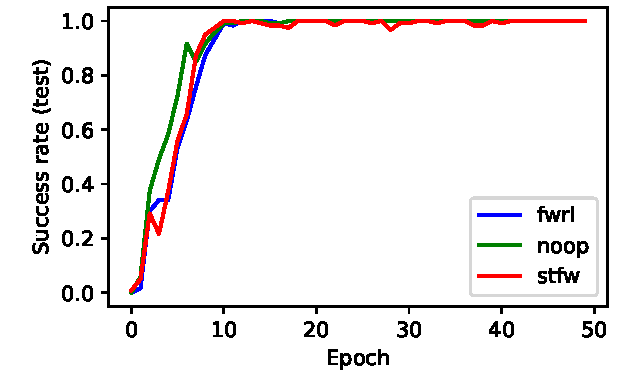
\includegraphics[width=\frac\columnwidth]{media/res/f0d4cfa-FetchReach-v1-stfw-none/test/success_rate.pdf}%
  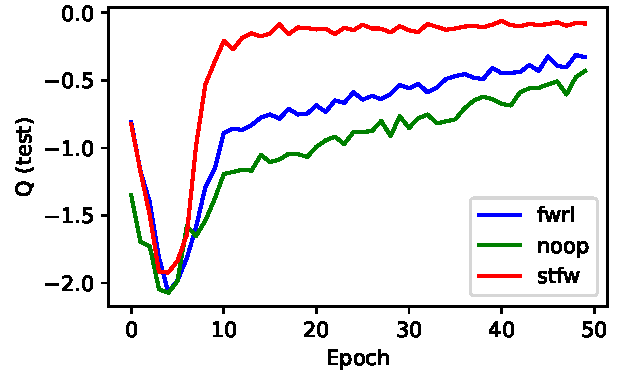
\includegraphics[width=\frac\columnwidth]{media/res/f0d4cfa-FetchReach-v1-stfw-none/test/mean_Q.pdf}%
  \includegraphics[width=\frac\columnwidth]{media/res/f0d4cfa-FetchReach-v1-stfw-none/train/critic_loss.pdf}%
  \includegraphics[width=\frac\columnwidth]{media/res/f0d4cfa-FetchReach-v1-stfw-none/train/critic_addnl_loss.pdf}\\
  \caption{
    stepfwrl = DDPG loss $\Loss_{\text{ddpg}}$ + Step loss $\Loss_{\text{step}}$
    + FWRL constraints $\Loss_{\text{upper}} + \Loss_{\text{lower}}$, noop =
    DDPG loss $\Loss_{\text{ddpg}}$  + HER
    sampling, fwrl = DDPG Loss $\Loss_{\text{ddpg}}$ + FWRL constraints $\Loss_{\text{upper}} + \Loss_{\text{lower}}$.
    All experiments on Fetch-Reach task.
  }%
  \label{fig:fwrl-stepfwrl-noop-FetchReach}%
\end{figure}%
% 

%
\begin{figure}%
  \def\frac{0.24}
  With HER sampling\\
  \includegraphics[width=\frac\columnwidth]{media/res/ea0e35b-FetchPush-v1-stfw-future/test/success_rate.pdf}%
  \includegraphics[width=\frac\columnwidth]{media/res/ea0e35b-FetchPush-v1-stfw-future/test/mean_Q.pdf}%
  \includegraphics[width=\frac\columnwidth]{media/res/ea0e35b-FetchPush-v1-stfw-future/train/critic_loss.pdf}%
  \includegraphics[width=\frac\columnwidth]{media/res/ea0e35b-FetchPush-v1-stfw-future/train/critic_addnl_loss.pdf}\\
  Without HER sampling\\
  \includegraphics[width=\frac\columnwidth]{media/res/ea0e35b-FetchPush-v1-stfw-none/test/success_rate.pdf}%
  \includegraphics[width=\frac\columnwidth]{media/res/ea0e35b-FetchPush-v1-stfw-none/test/mean_Q.pdf}%
  \includegraphics[width=\frac\columnwidth]{media/res/ea0e35b-FetchPush-v1-stfw-none/train/critic_loss.pdf}%
  \includegraphics[width=\frac\columnwidth]{media/res/ea0e35b-FetchPush-v1-stfw-none/train/critic_addnl_loss.pdf}%
  \caption{stepfwrl = DDPG loss $\Loss_{\text{ddpg}}$ + Step loss $\Loss_{\text{step}}$
    + FWRL constraints $\Loss_{\text{upper}} + \Loss_{\text{lower}}$, noop =
    DDPG loss $\Loss_{\text{ddpg}}$  + HER
    sampling, fwrl = DDPG Loss $\Loss_{\text{ddpg}}$ + FWRL constraints $\Loss_{\text{upper}} + \Loss_{\text{lower}}$.
    All experiments on Fetch-Push}
  \label{fig:loss-func-fetch-push}
\end{figure}
%

%
\begin{figure}
  \def\frac{0.32}
Loss function breakdown without HER sampling on Fetch Push\\
  \includegraphics[width=\frac\columnwidth]{media/res/f84daa7-FetchPush-v1-stfw-none/test/success_rate.pdf}%
  \includegraphics[width=\frac\columnwidth]{media/res/f84daa7-FetchPush-v1-stfw-none/test/mean_Q.pdf}%
  \includegraphics[width=\frac\columnwidth]{media/res/f84daa7-FetchPush-v1-stfw-none/train/critic_loss.pdf}\\
Loss function breakdown with HER sampling on Fetch Push\\
  \includegraphics[width=\frac\columnwidth]{media/res/3f1eafe-FetchPush-v1-stfw-future/test/success_rate.pdf}%
  \includegraphics[width=\frac\columnwidth]{media/res/3f1eafe-FetchPush-v1-stfw-future/test/mean_Q.pdf}%
  \includegraphics[width=\frac\columnwidth]{media/res/3f1eafe-FetchPush-v1-stfw-future/train/critic_loss.pdf}%
  \caption{
    Fetch Push results. Loss function changes do no seem to make a difference.
    There are four parts to the loss function (1) DDPG Loss $\Loss_{\text{ddpg}}$ ,
    (2) Step loss$\Loss_{\text{step}}$,  
    (3) Lower bound $\Loss_{\text{lower}}$ and
    (4) Upper bound $\Loss_{\text{upper}}$ .
    ddpg = $\Loss_{\text{ddpg}}$,
    dqst = $\Loss_{\text{ddpg}}$ + $\Loss_{\text{step}}$,
    fwrl = $\Loss_{\text{ddpg}}$ + $\Loss_{\text{lower}}$ +
    $\Loss_{\text{upper}}$,
    qlst = $\Loss_{\text{ddpg}}$ + $\Loss_{\text{step}}$ + $\Loss_{\text{lower}}$ + $\Loss_{\text{upper}}$.
    stfw = $\Loss_{\text{step}}$ + $\Loss_{\text{lower}}$ + $\Loss_{\text{upper}}$,
    stlo = $\Loss_{\text{step}}$ + $\Loss_{\text{lower}}$,
    stup = $\Loss_{\text{step}}$ + $\Loss_{\text{upper}}$.
    Success rate is the fraction of times the agent reaches the goal. Q(test) is
    the estimated cumulative reward by the network. Critic loss is the total
    loss plotted during training.
    Because stfw, stlo, stup fail to succeed, we infer that the $\Loss_{\text{ddpg}}$ DDPG loss is
    critical for making the algorithm work. Since the qlst works better than
    fwrl, we infer that $\Loss_{\text{step}}$ Step loss is also important.
    only.
    Since there is slight improvement in dqst over ddpg, this means
    $\Loss_{\text{step}}$ really helps. dqst did not run fully but it shows
    promise (I need to fix a bug).
    But why does the loss for stfw keep rising? Does it mean that the SGD is not
    able to optimize the loss gradients in the right direction?
  }%
  \label{fig:fwrl-stepfwrl-noop-FetchPush}%
\end{figure}%
% 

%
\begin{figure}
  \def\frac{0.32}
  On Fetch Push\\
  \includegraphics[width=\frac\columnwidth]{media/res/38f4625-FetchPush-v1-fwrl-future/test/success_rate.pdf}%
  \includegraphics[width=\frac\columnwidth]{media/res/38f4625-FetchPush-v1-fwrl-future/test/mean_Q.pdf}%
  \includegraphics[width=\frac\columnwidth]{media/res/38f4625-FetchPush-v1-fwrl-future/train/critic_loss.pdf}\\
  On Fetch Reach\\
  \includegraphics[width=\frac\columnwidth]{media/res/38f4625-FetchReach-v1-fwrl-future/test/success_rate.pdf}%
  \includegraphics[width=\frac\columnwidth]{media/res/38f4625-FetchReach-v1-fwrl-future/test/mean_Q.pdf}%
  \includegraphics[width=\frac\columnwidth]{media/res/38f4625-FetchReach-v1-fwrl-future/train/critic_loss.pdf}\\
  On Fetch Slide\\
  \includegraphics[width=\frac\columnwidth]{media/res/38f4625-FetchSlide-v1-fwrl-future/test/success_rate.pdf}%
  \includegraphics[width=\frac\columnwidth]{media/res/38f4625-FetchSlide-v1-fwrl-future/test/mean_Q.pdf}%
  \includegraphics[width=\frac\columnwidth]{media/res/38f4625-FetchSlide-v1-fwrl-future/train/critic_loss.pdf}%
  On Fetch Pick and Place\\
  \includegraphics[width=\frac\columnwidth]{media/res/38f4625-FetchPickAndPlace-v1-fwrl-future/test/success_rate.pdf}%
  \includegraphics[width=\frac\columnwidth]{media/res/38f4625-FetchPickAndPlace-v1-fwrl-future/test/mean_Q.pdf}%
  \includegraphics[width=\frac\columnwidth]{media/res/38f4625-FetchPickAndPlace-v1-fwrl-future/train/critic_loss.pdf}%
  On HandReach\\
  \includegraphics[width=\frac\columnwidth]{media/res/38f4625-92450888-HandReach-v0-fwrl-future/test/success_rate.pdf}%
  \includegraphics[width=\frac\columnwidth]{media/res/38f4625-92450888-HandReach-v0-fwrl-future/test/mean_Q.pdf}%
  \includegraphics[width=\frac\columnwidth]{media/res/38f4625-92450888-HandReach-v0-fwrl-future/train/critic_loss.pdf}%
  \caption{
    Fetch results. Loss function changes do no seem to make a difference.
    There are four parts to the loss function (1) DDPG Loss $\LossDDPG$ ,
    (2) Step loss$\LossStep$,  
    (3) Lower bound $\LossLo$ and
    (4) Upper bound $\LossUp$ .
    ddpg = $\LossDDPG$,
    dqst = $\LossDDPG$ + $\LossStep$,
    fwrl = $\LossDDPG$ + $\LossLo$ +
    $\LossUp$,
    qlst = $\LossDDPG$ + $\LossStep$ + $\LossLo$ + $\LossUp$,
    dqte = $\LossDDPG$ + $\LossTrieq$,
    qste = $\LossDDPG$ + $\LossStep$ + $\LossTrieq$.
    Success rate is the fraction of times the agent reaches the goal. Q(test) is
    the estimated cumulative reward by the network. Critic loss is the total
    loss plotted during training.
    Because stfw, stlo, stup fail to succeed, we infer that the $\LossDDPG$ DDPG loss is
    critical for making the algorithm work. Since the qlst works better than
    fwrl, we infer that $\LossStep$ Step loss is also important.
    only.
    Since there is slight improvement in dqst over ddpg, this means
    $\LossStep$ really helps. dqst did not run fully but it shows
    promise (I need to fix a bug).
    But why does the loss for stfw keep rising? Does it mean that the SGD is not
    able to optimize the loss gradients in the right direction?
  }%
  \label{fig:fwrl-stepfwrl-noop-FetchPush}%
\end{figure}%
% 

%
\begin{figure}%
  \def\frac{0.25}
  \includegraphics[width=\frac\columnwidth]{media/res/3d07a6e-FetchReachPR-v1-fwrl-future/test/success_rate.pdf}%
  \includegraphics[width=\frac\columnwidth]{media/res/3d07a6e-FetchReachPR-v1-fwrl-future/test/mean_Q.pdf}%
  \includegraphics[width=\frac\columnwidth]{media/res/3d07a6e-FetchReachPR-v1-fwrl-future/test/ag_g_dist.pdf}%
  \includegraphics[width=\frac\columnwidth]{media/res/3d07a6e-FetchReachPR-v1-fwrl-future/train/critic_loss.pdf}%
  \label{fig:path-rewards}%
  \caption{Experiment to see the effect of only path rewards on loss terms. We
    did not include a step term which becomes very important in this case.}%
\end{figure}%
% 

%
\begin{figure}%
  \def\frac{0.24}
  \includegraphics[width=\frac\columnwidth]{./media/res/04a8fc6-814a3d24-FetchSlide-v1-fwrl-future/test/success_rate.pdf}%
  \includegraphics[width=\frac\columnwidth]{./media/res/04a8fc6-814a3d24-FetchSlide-v1-fwrl-future/test/mean_Q.pdf}%
  \includegraphics[width=\frac\columnwidth]{./media/res/04a8fc6-814a3d24-FetchSlide-v1-fwrl-future/test/ag_g_dist.pdf}%
  \includegraphics[width=\frac\columnwidth]{./media/res/04a8fc6-814a3d24-FetchSlide-v1-fwrl-future/train/critic_loss.pdf}%
  \label{fig:loss-term-weights}%
  \caption{Effect of weighted combination of loss terms on FetchSlide. The three
  loss terms being weighed in order are $[\LossDDPG, \LossLo, \LossUp]$}%
\end{figure}%
% 
We compared weighted combination of loss terms

%
\begin{figure}%
  \def\frac{0.24}
  \includegraphics[width=\frac\columnwidth]{media/res/d249d2d-c9bfa98b-FetchPush-v1-fwrl-future/test/success_rate.pdf}%
  \includegraphics[width=\frac\columnwidth]{media/res/d249d2d-c9bfa98b-FetchPush-v1-fwrl-future/test/mean_Q.pdf}%
  \includegraphics[width=\frac\columnwidth]{media/res/d249d2d-c9bfa98b-FetchPush-v1-fwrl-future/test/ag_g_dist.pdf}%
  \includegraphics[width=\frac\columnwidth]{media/res/d249d2d-c9bfa98b-FetchPush-v1-fwrl-future/train/critic_loss.pdf}%
  \label{fig:middle-vs-uniform}%
  \caption{Effect of choosing the intermediate sample in the \emph{middle} of the
    trajectory vs \emph{uniform}ly random in the trajectory on FetchPush}%
\end{figure}%
% 

%
\begin{figure}%
  \includegraphics[width=\columnwidth]{./media/res/eb45946-path_reward-FetchSlidePR-v1-dqst/test/success_rate.pdf}%
  \label{fig:}%
  \caption{Effect of path rewards on FetchSlide}%
\end{figure}%
% 

%\subsection{Unanswered questions and things to try}
%
%\subsubsection{FWRL specific sampling}
%Right now the shuffle step in the algorithm is totally random and probably
%introduces more noise in the algorithm than it helps. A modification of HER
%sampling would sampling three time steps from the trajectory (single episode)
%$t_1 > t_2 > t_3$ and use $t_2$ as the intermediate state for
%$\LossUp$ and $\LossLo$.
%
%
%\subsubsection{Why is any loss term with upper/lower worse?}
%This is probably answered by  the above section but what are the other
%explanations. The total ``Critic loss'' is increasing for stfw
%($=\LossStep$ + $\LossLo$ + $\LossUp$),
%which seems to say that with $\LossDDPG$, it is hard to optimize the functions.
%
%
%\subsection{Is it still a contribution if the upper and lower bounds do not
%  improve the results?}
%Can we claim that this alternative formulation is new and more principled than HER?
\end{document}
